%\chapter{Bayesian Neural Networks for Cancer Types Prediction}
%\chapter{Neuro-symbolic Representation Learning on Knowledge Graphs}
\chapter{Symbolic Decision Reasoning}\label{chapter:nsr}
\textit{``Your statistical track record for decision-making is somewhat concerning.''}- Jennifer Lynn Barnes, All In\\

\section{Chapter Overview}
%\section{Symbolic reasoning}
%In the previous chapter, a surrogate model is trained to deduce a rule set to explain individual diagnostic decision~(i.e., cancer type and subtype) to end users. 
The model\footnote{It is considered as the Oracle model.} based on multimodal convolutional autoencoder~(MCAE) classifier can predict the cancer types and subtypes with a high level of confidence. Besides, a surrogate model is trained to deduce a rule set to explain individual diagnostic decision~(i.e., cancer type and subtype) to end users. However, many efficient ML models that may be better at predicting, detecting, and processing patterns than human, but may not be able to reason its decision~\cite{miller2018explanation}.
Similarly, both the MCAE and the surrogate model are incapable of explaining if the features~(i.e., marker genes) in the antecedents are biologically significant. One of the main reasons for this is that no domain knowledge is incorporated into the models~(i.e., both oracle and surrogate models). In other words, all the machine learning~(ML) models are trained on training data and clinical outcome and subsequently optimized based on a set of statistical learning theory. % and a bunch of hyperparameters. 

\hspace*{3.5mm} In cancer diagnosis, it is not only the necessity to accurately predict the cancer types, but also understanding its biological meaning is important. %An AI system based on ``black-box'' methods are incapable in the advancement of science with only numbers, not insight?
On the other hand, one of the first steps to improve the performance of a decision support system~(DSS) is to understand its weaknesses. Weakness analysis on `black-box' ML models is not straightforward as interpretable models~\cite{bhatt2020explainable}. The better we understand how and why an ML model works~(e.g., which factors caused it to make predictions), why it fails in certain cases~(e..g, which factors caused it to make wrong predictions), the easier it becomes to improve it~\cite{miller2018explanation}. 
In a sensitive clinical setting where the impact of AI on human life is relevant, e.g., medical diagnoses, explainability is not only a desirable property but also became a legal requirement with the EU GDPR~\cite{karmakar2019tight}. In addition to predictions and explanations, reasoning capability is desirable such that a model can reason about entities and eventually answer queries posed by human operators in order to guide decision making processes accurate, interactive, and trustworthy.  

%For a clinical DSS In a clinical setting, two more questions evolved: i) why should a physicians, for example, trust the provided diagnosis decision?, ii) will `black-box' methods contribute to advancement of science with only numbers, not insight? 

\hspace*{3.5mm} Structured and unstructured data, knowledge, and facts about drugs, genes, protein, viruses, and their mechanism are spread across a huge number of scientific articles. These articles form a large-scale knowledge source and can have a huge impact in disseminating knowledge about mechanism of carcinogenics. A knowledge graph~(KG) can be built by integrating such knowledge, facts, and data, which can be used to introduce necessary semantics into a DNN to aid in diagnosing cancer. 
Based on these motivations, this chapters focuses on extracting and integrating cancer related knowledge into a domain-specific KG. Then the ontological reasoning~(OR) is applied to infer and validate domain knowledge about top-k biomarkers that were identified and used in the previous chapters. % to generate human-interpretable decision rules. 

\section{Introduction}
Humans communicate with signs and symbols, what we desire from machines too~\cite{SAI}. Combinations of symbols that express their interrelations is refereed as reasoning. When humans combine a bunch of signs together to express something meaningful, it is know as ``symbolic manipulation''~\cite{alirezaie2019semantic}. However, in many scientific process, `proof' simply doesn't exist; there can only be facts and evidence that can lead us to certain conclusions~\cite{SAI,tolstoy2005death}. In such a situation, deductive or inductive reasoning technique is used to reach a logical and true conclusion or to express complex thought based on symbolic relations. For example, the old Roman chestnut: \textit{``All men are mortal; Caius is a man; therefore, Caius is mortal''}~\cite{tolstoy2005death}. 
%, e.g., the old Roman chestnut: \texttt{`All men are mortal; Caius is a man; therefore Caius is mortal'}.%
%\subsubsection{Neuro-symbolic reasoning}
%Humans usually communicate with signs and symbols, what we desire from machines too~\cite{SAI}. Combinations of symbols that express their interrelations is refereed as reasoning. When humans combine a bunch of signs together to express something meaningful, we call it symbolic manipulation~\cite{alirezaie2019semantic}. 
%However, in many scientific process, `proof' simply doesn't exist; there can only be facts and evidence that can lead us to certain conclusions. In such a case, either deductive or inductive reasoning is used to reach a specific logical and true conclusion or to express complex thought based on symbolic relations, e.g., the old Roman chestnut: \texttt{`All men are mortal; Caius is a man; therefore Caius is mortal'}~\cite{tolstoy2005death}. 
A more practical example can be introduced as follows: suppose a man named John is very hungry. Assuming John likes pizza, but he is a vegetarian. John went to a nearby restaurant and asked the waiter for an option for the vegetarian, preferably a vegetable pizza. The waiter replies ``I'm not sure, if we have such an option, but, Margherita pizza could be suitable for the vegetarian''. 
%How will you be sure that the waiter is right? Well, the simplest answer to this question would be 
After reading the ingredients and based on his instincts, John reached a logical conclusion that the waiter was right. The symbols and the ``symbolic manipulation'' utilized by John can be described in natural language, as shown in \cref{fig:sparqlEx11}.   

%\vspace{-4mm}
%{\scriptsize \texttt{\\`Vegetarian pizza is one kind of pizza.\\ Margherita pizza is one type of pizza.\\ Tomato topping is one type of vegetable topping. \\Mozzarella topping is one type of cheese topping. \\Vegetarian pizza made of both vegetable and cheese topping.\\ Margherita pizza has either mozzarella~(or tomato) topping or both.\\ Therefore, Margherita is a vegetarian pizza'.}}

\begin{figure}[h]
    \centering
    \scriptsize
    \begin{Verbatim}[frame=single,numbers=left]
        Vegetarian pizza is one type of pizza; 
        Margherita pizza is one type of pizza;
        Tomato topping is one type of vegetable topping;
        Mozzarella topping is one type of cheese topping;
        Vegetarian pizza made of both vegetable and cheese topping;
        Margherita pizza has either mozzarella~(or tomato) topping or both;
        Therefore, Margherita pizza is a vegetarian pizza.
    \end{Verbatim}
    \vspace{-3mm}
    \caption{Deriving a new logical conclusion based on given facts and knowledge}
    \label{fig:sparqlEx11}
\end{figure}

\hspace*{3.5mm} However, for a machine deriving such a logical conclusion is always subject to the availability of prior facts and knowledge. Since ontologies and rules can be used to define and reason about the semantics of the terms used in a KG~\cite{hogan2020knowledge}, ontological reasoning, in the form of symbolic reasoning can infer simple to complex rules~\cite{futia2020integration}. In particular, based on a set of prior facts and evidence from a domain-specific ontology~(e.g., a Pizza ontology), an ontology reasoner can infer, a logical conclusion in the form of description logic axioms~(DLx), as shown in \cref{fig:pizza11}. %, which we will see in the next subsection. 

\begin{figure*}[h]
	\centering
	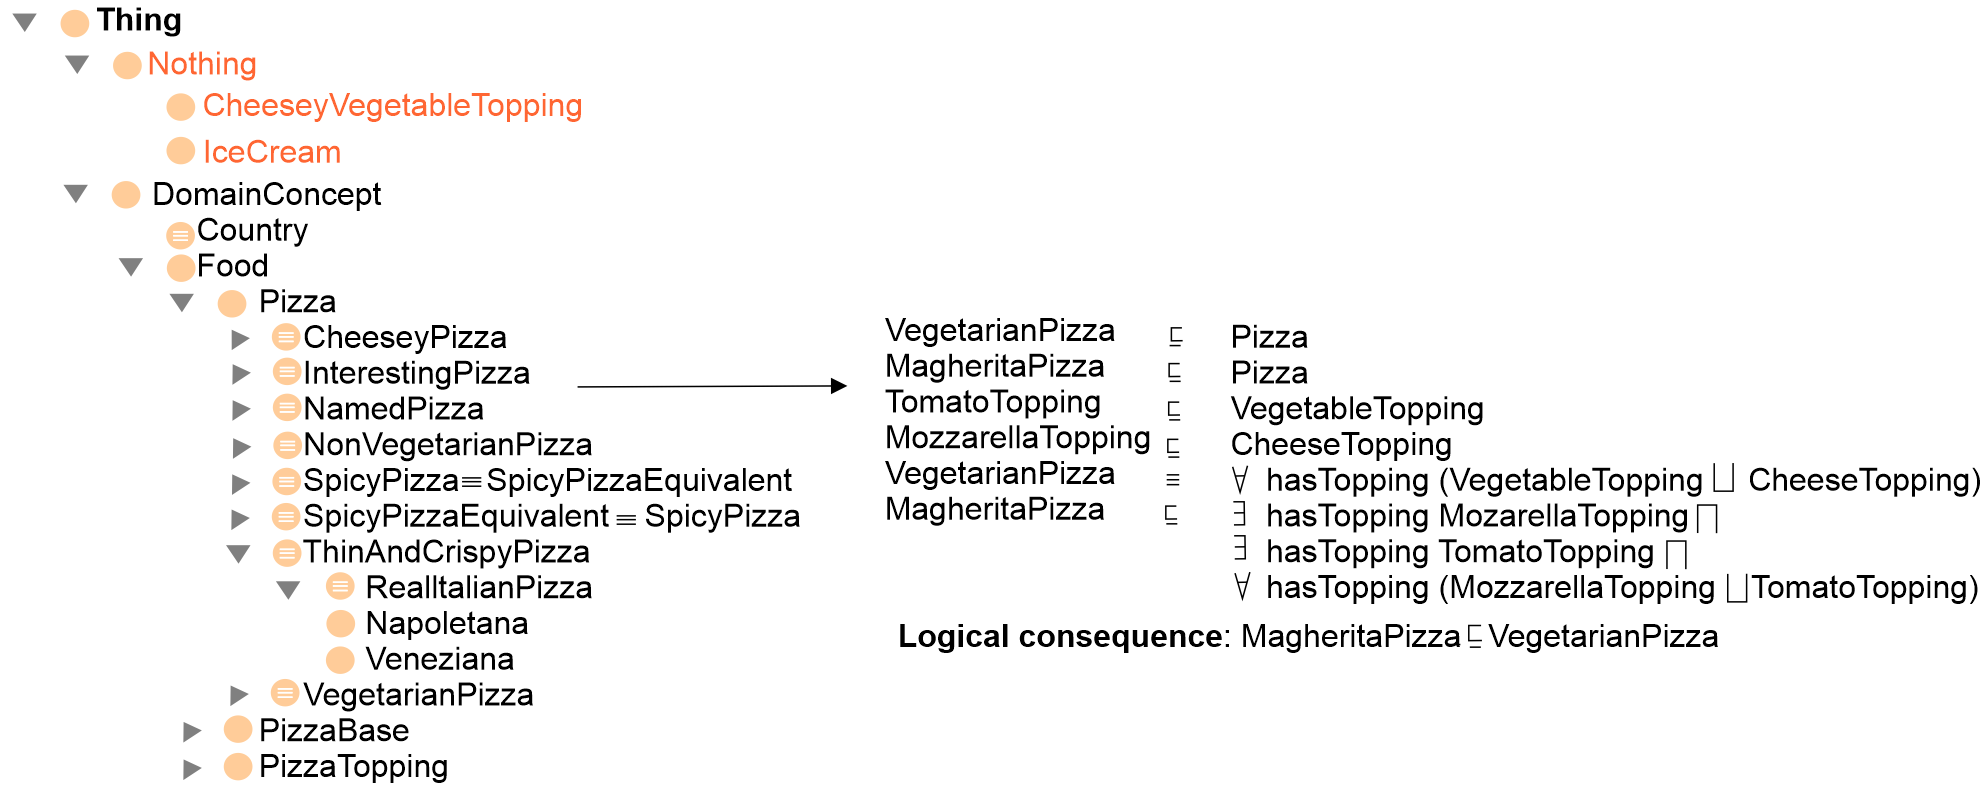
\includegraphics[scale=0.65]{images/pizza_onto.png}
	\caption{Example of inferencing logical conclusion that Margherita is a vegetable pizza.} 
	\label{fig:pizza11}
	\vspace{-2mm}
\end{figure*}

%\subsubsection{Deductive reasoning} 
\hspace*{3.5mm} Both deductive and inductive reasoning techniques are used to reach logical conclusion. Deductive reasoning is a basic form of valid reasoning in which the deduction starts with a general statement. Then, all the possibilities are checked to reach a logical conclusion. Scientific methods often use deduction to test hypotheses and theories. In deductive inference, a theory is hold, followed by predicting the observations if the theory was correct. Conclusions are also often drawn similar to what we do based on mathematics from a logical syllogism. Deductive reasoning usually involves: a premise, followed by one or more premise, and finally an inference. For example, \textit{``All oncogenes are responsible for cancer; TP53 is a oncogene; therefore, TP53 is responsible for cancer''}. In this example, first two premises are followed by a conclusion. In deductive reasoning, the conclusion will be correct if all the statements are correct in which the inferencing and reasoning are defined as follows~\cite{hogan2020knowledge}: 

\begin{itemize}[noitemsep]
    \item \textbf{Inference} - is the derivation of new knowledge from existing knowledge and axioms. Based on a set of axioms and explicit facts, a reasoner is able to derive implicit, but previously unknown facts. 
    \item \textbf{Reasoning} - is deciding whether a propositional formula is satisfiable or not. Reasoning task is carried out via a search process involving multiple inferences.
\end{itemize}

%\subsubsection{Inductive reasoning} 
\hspace*{3.5mm} On the other hand, often symbols also express lessons that we derive inductively based on domain knowledge or real-world experiences. That is, inductive reasoning is the opposite of deductive reasoning in which a broad generalizations is made from specific observations~\cite{hogan2020knowledge}. In real-life, human make many observations, discern a pattern, make a generalization, and infer an explanation or a theory. Similarly, using inductive reasoning, specific observations can be made to draw a general conclusion. For example, \textit{``Oncogenes are responsible for cancer, don't apply gene silencing blindly''}. 
However, the downside of inductive reasoning is that it can end up with a false conclusion, even if all of the premises are true in a statement. For example, \textit{``TCF3 is an oncogene; TCF3 has tumor-suppressor functionality; all oncogenes have tumor-suppressor functionality''}. Since only the proto-oncogenes have tumor-suppressor functionality, this conclusion is not biologically correct.

%\hspace*{3.5mm} %\hspace*{3.5mm}  However, in many scientific process, `proof' simply doesn't exist; there can only be facts and evidence that can lead us to certain conclusions~\cite{SAI,tolstoy2005death}. In such a case, either deductive or inductive reasoning is used to reach a specific logical and true conclusion or to express complex thought based on symbolic relations, e.g., the old Roman chestnut: \texttt{`All men are mortal; Caius is a man; therefore Caius is mortal'}. 
\hspace*{3.5mm} In the symbolic AI approach~(also known as Good Old-Fashioned Artificial Intelligence~(GOFAI) - a dominant paradigm during 1980s), where booth deductive and inductive reasoning techniques were used, symbols are elements of a \textit{`lingua franca'} between humans and deep neural networks~(DNN)~\cite{janssens2007dynamic}. However, since contemporary explainability techniques mostly adjust the weights and measures model inputs to determine their effects on outputs, many AI practitioners merely consider symbolic AI systems as the first step towards achieving a true XAI system. 
Subsequently, the neuro-symbolic AI paradigm has emerged, which combines DNNs with symbolic-AI~\cite{futia2020integration}.  %In this paper, authors utilized knowledge representation using symbolic logic and automated reasoning to generate embeddings of nodes using neural networks, which encodes related information in knowledge graphs(KGs). 
 % in which reasoning based on a domain-specific ontology help increase interpretability of the ML model.
To develop such neuro-symbolic AI system, a domain-specific KG, an interpretable ML model, and an explainable interface are most important components. 

\hspace*{3.5mm} Besides, the ML model has to be capable of learning the probabilistic correlations from the KG, as well as abstract and higher-order concepts from the data~\cite{SAI}. Once those factors are identified, explaining: i) the decision reasoning~(i.e., via an explainable interface), ii) they way how the model produced the decision in a certain way, by enumerating w.r.t rules can make even a complex DNN model highly transparent. In such a situation, symbolic reasoning can codify intricate explanations of results of ML models into sustainable rules that are more transparent and reliable in critical domains~\cite{futia2020integration}. Since decision rules are more effective at explaining diagnosis decisions in clinical setting, they align with EU GDPR algorithmic transparency and right to explanation~\cite{kaminski2019right}.
%What makes the KB side of AI so influential in recent years is that the 
These assumptions are backed up by the fact that rules are repeatable, consistently producing the same output, whereas ML model's outputs are not deterministic, which is due to stochastic nature of the model\footnote{The output could be different across runs}~\cite{karim2019onconetexplainer})~\cite{alshahrani2017neuro}.
  % such as healthcare,
%. Unlike ML, semantic inferencing of the KB side of AI understands the meaning of its processing results, 

\begin{sidewaysfigure}
	\centering
	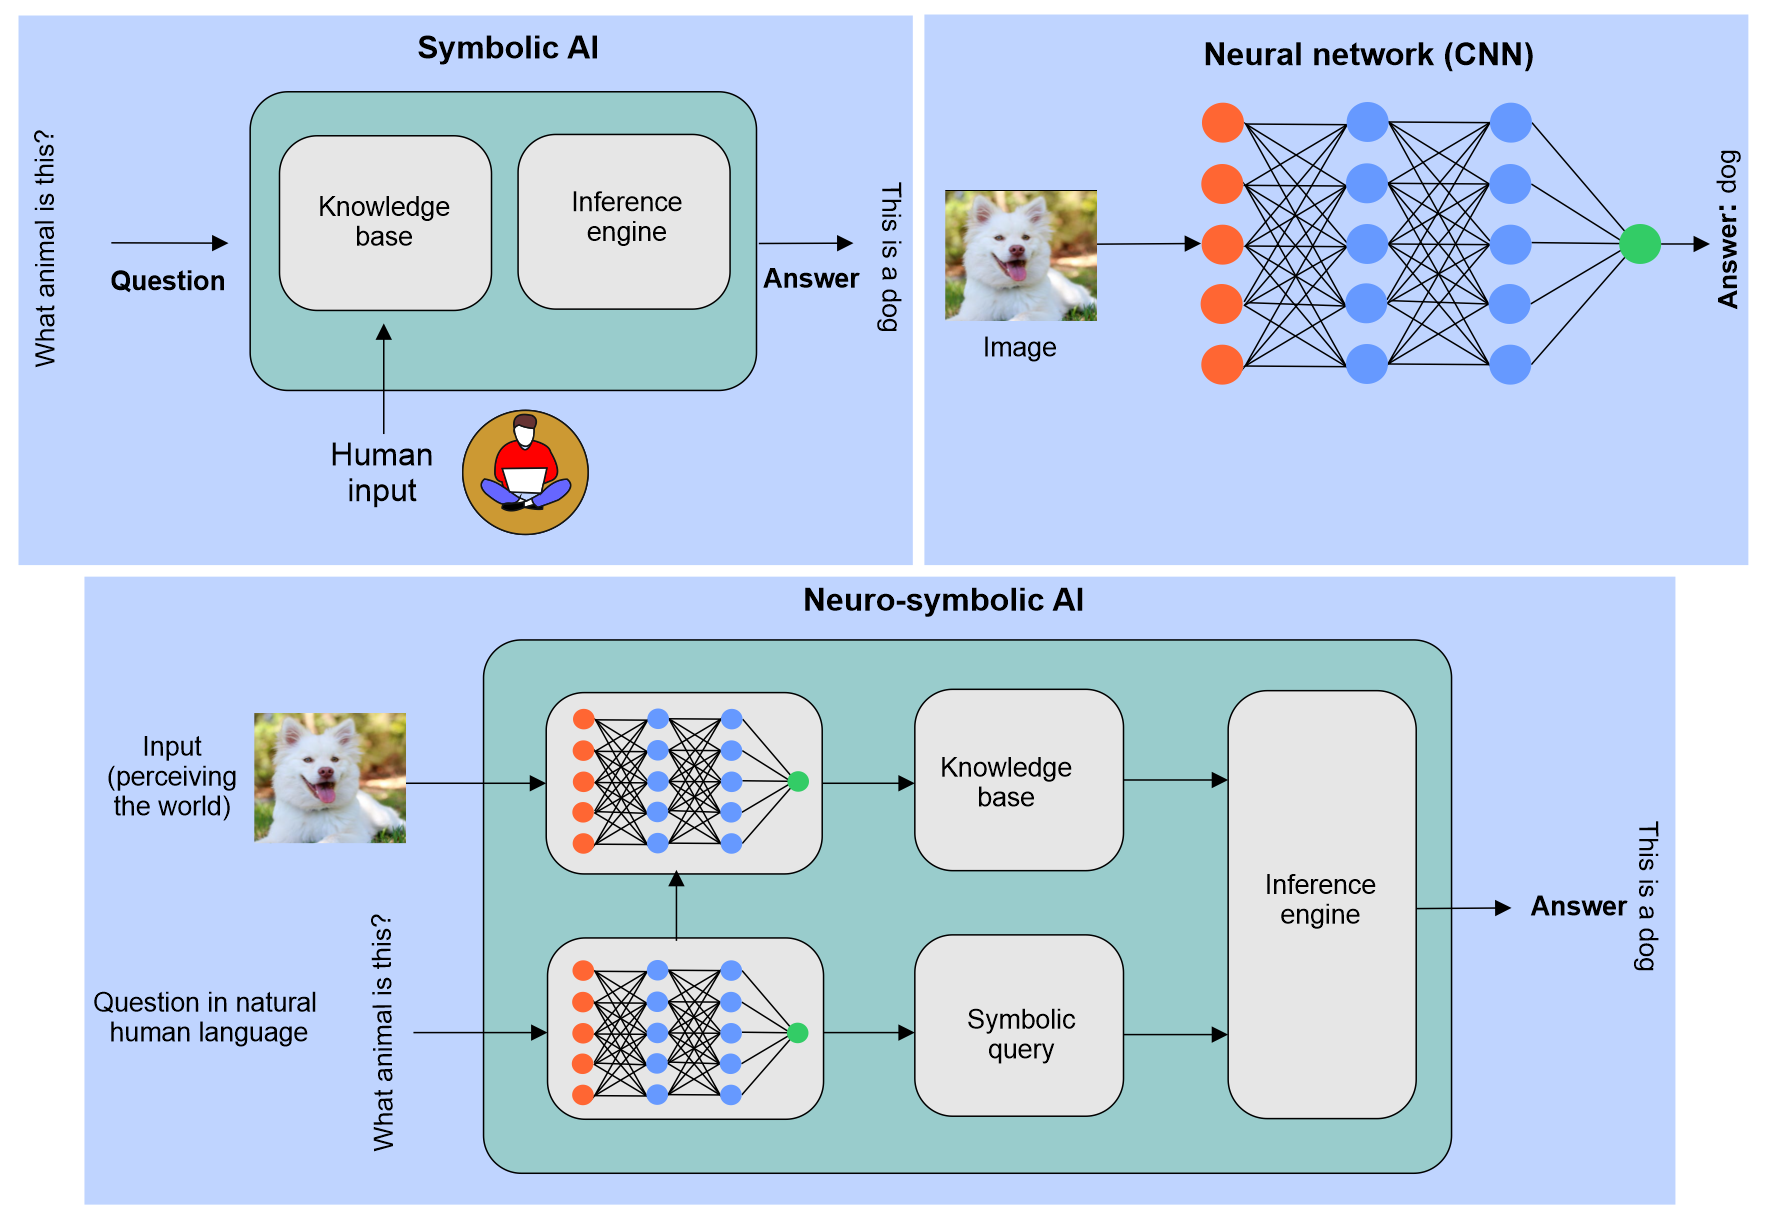
\includegraphics[scale=0.9]{images/Capture5.PNG}
	\caption[Symbolic vs. A neuro-symbolic AI]{A hybrid approach, conceptually recreated based on the by Anil Ananthaswamy et al~\cite{AIsnextbigleap} is known as neuro-symbolic AI. A neuro-symbolic AI system combines both symbolic AI~(upper left - where a human develops ``knowledge bas'' that the system uses to answer questions) and neural networks~(upper right) that are trained to provide the answers. During training, a DNN adjusts the strength of the connections between layers of nodes. In a hybrid AI system, human is replaced with a DNN, to generate only those portions of the knowledge base that it needs to answer a given question.}
	\label{fig:neurosymbolic_AI}
	\vspace{-2mm}
\end{sidewaysfigure} 

\hspace*{3.5mm} SW address data variety, by proposing graphs as a unifying data model, to which a data source can be mapped in the form of a graph structure, where an ontology defines the relationships between concepts~\cite{hitzler2009foundations}. An ontology provides a formal representation of domain-specific entities\cite{alirezaie2019semantic}. Ontologies are semantic data models that define the types of things that exist in a domain and the properties that can be used to describe them, including the relationships between them~\cite{hogan2020knowledge}. A graphs may not only contain data, but also metadata and domain knowledge~(ontologies containing axioms or rules), all in the same uniform structure, and are then called knowledge graph\footnote{~Ontology + data = knowledge graph}~(KGs)~\cite{wilcke2017knowledge,hogan2020knowledge}.
%Such knowledge structure not only contain data, but also metadata and domain knowledge~(ontologies containing axioms or rules), all in the same uniform structure, and are then called knowledge graphs\footnote{Ontology + data = knowledge graph.}~(KGs)~\cite{wilcke2017knowledge,hogan2020knowledge}. 
% KGs are typically represented in the standardized RDF\footnote{Resource Description Framework: \url{https://www.w3.org/RDF/}} data model and queried using the SPARQL Protocol and RDF Query Language.

\hspace*{3.5mm} Hogan et al.~\cite{hogan2020knowledge} defines KG as \textit{a graph of data intended to accumulate and convey knowledge of the real world, whose nodes represent entities of interest and whose edges represent potentially different relations between these entities}. Nonakatakeuchi et al.~\cite{nonakatakeuchi1995} called ``something that is known and can be written down'' as ``\textit{explicit knowledge}''. That is, knowledge may be composed of simple statements, as in the previous example: \textit{``TP53 is a oncogene''}, or quantified statements, such as \textit{``All oncogenes are responsible for cancer''}. Simple statements can be accumulated as edges in a KG, while quantified statements provide more expressive way to represent knowledge, which however requires \textit{ontologies}~\cite{hogan2020knowledge}. \textit{Deductive reasoning} can then be used to entail and accumulate extended knowledge such as \textit{``TP53 is responsible for cancer''}. Moreover, knowledge can be extracted from external sources like scientific articles. 

\hspace*{3.5mm} Eventually, a KG is an effective means for capturing and structuring a large -scale data from various heterogeneous sources. In a KG, nodes represent entities and edges represent binary relations between those entities~\cite{hogan2020knowledge}. More formally, a KG can be defined as $G=\{E,R,T\}$, where $G$ is a labeled and directed multi-graph, and $E, R, T$ are the sets of entities, relations, and triples, respectively. Each triple is formalized as $(u,e,v) \in T$, where $u \in E$ is the head node, $v \in E$ is the tail node, and $e \in R$ is the edge connecting $u$ and $v$~\cite{hogan2020knowledge}. \Cref{fig:cancer_ontology_example} shows a high-level cancer KG, which connects knowledge, facts, and data about the disease cancer. Following explicit relations are defined in the KG: 

\begin{figure*}[h]
	\centering
	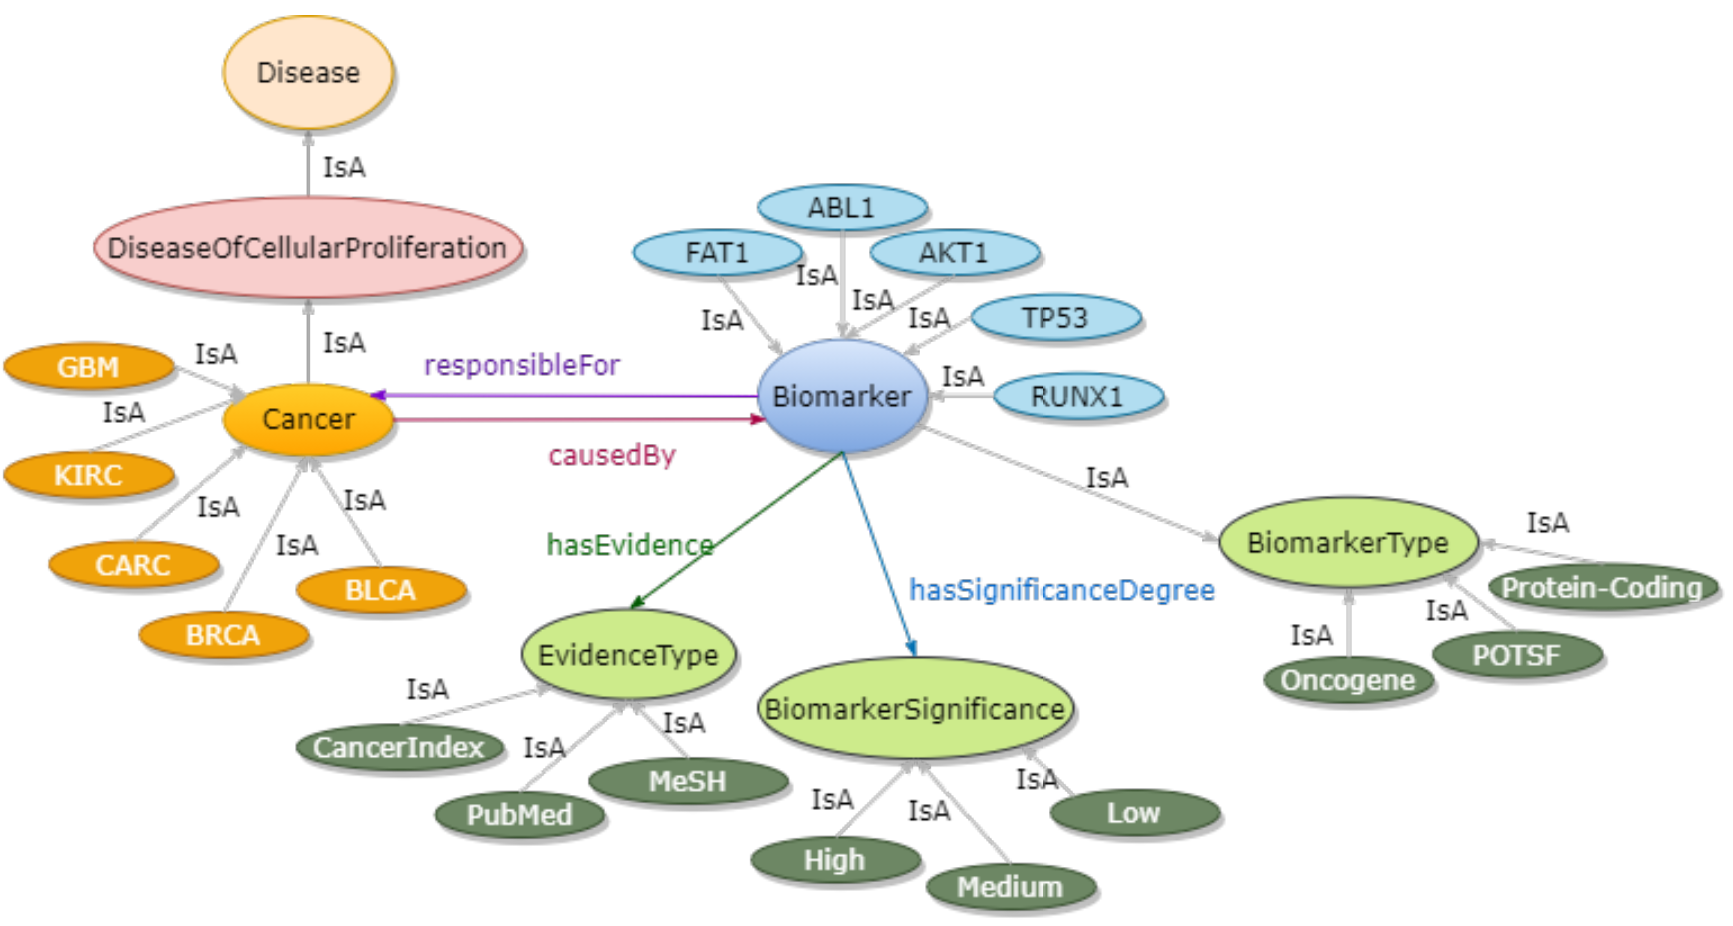
\includegraphics[scale=0.65]{images/cancer_ontology_example.png}
	\caption{An example knowledge graph that connects knowledge, facts, and data about cancer} 
	\label{fig:cancer_ontology_example}
	\vspace{-2mm}
\end{figure*}

\begin{itemize}[noitemsep]
\scriptsize{
    \item ``Cancer'' is a ``DiseaseOfCellularProliferation''~(i.e., disease of cellular proliferation)
    \item ``DiseaseOfCellularProliferation' is of type ``Disease'', but biologically a unifying concept that excessive proliferation of cells and turnover of cellular matrix contribute significantly to the pathogenesis of several diseases, including cancer, atherosclerosis, rheumatoid arthritis, psoriasis, idiopathic pulmonary fibrosis, scleroderma and cirrhosis of the liver~\cite{sporn1981proliferative}.
    \item ``Cancer'' is caused by different gene ``Biomarkers''~(e.g., TP53), which also signify that ''Biomarkers'' are responsible for different types of cancers~(e..g, breast cancer -BRCA). 
    \item It is evident that a ``Biomarker'' is well-studied in scientific articles~(e.g., PubMed, MeSH, etc.)
    \item A ``Biomasrker'' has qualitative significance~(e.g., high, medium, low) w.r.t a certain cancer type
    \item A ``Biomarker'' can be categorized into oncogene, protein-coding gene, or protein-suppressor oncogene. 
    }
\end{itemize}

\hspace*{3.5mm} The above KG is consisting of as a set of nodes such as \gnode{Disease}, \gnode{Cancer}, \gnode{Biomarker}, \gnode{BiomarkerType}, \gnode{EvidenceType} and a set of edges between those nodes, such as \gedge{TP53}{isA}{Biomarker}, \gedge{BRCA}{isA}{Cancer}, \gedge{Cancer}{causedBy}{Biomarker}. 
A large-scale KG can have billions of linked entities expressing their relationships, where each node represent an entity and each edge signifies a semantic relationship between entities~\cite{karim2019drug}. Scientific literature and patents provide a huge treasure of structured and unstructured information about different biological entities. For example, PubMed is an essential resource for the medical domain~\cite{xu2020building}, which contain millions of scientific articles. A recent study by Reyes et al.~\cite{reyes2017proportion} found that the proportion of cancer-related entries in PubMed has risen from 6\% in the 1950s to 16\% in 2016. 

However, extracting knowledge and facts from unstructured, heterogeneous, and scattered sources is a very challenging task. Information extraction is the process of automatically extracting structured knowledge and facts from such unstructured and/or semi-structured machine-readable documents and other electronically represented sources~\cite{Liddy.2001}. Information extraction is typically divided into multiple subtasks~\cite{Jurafsky.2014} like entity extraction, named entity recognition~(NER), and relation extraction, as shown in \cref{fig:IE_pipeline}. Relation extraction also involves relation classification, which is typically formulated as a classification problem to classify the relationship between the entities identified in the text~\cite{xue2019fine}. A classifier takes a piece of text and two entities as inputs and predicts possible relations between the entities as output. 

\begin{figure}[h]
    \centering
    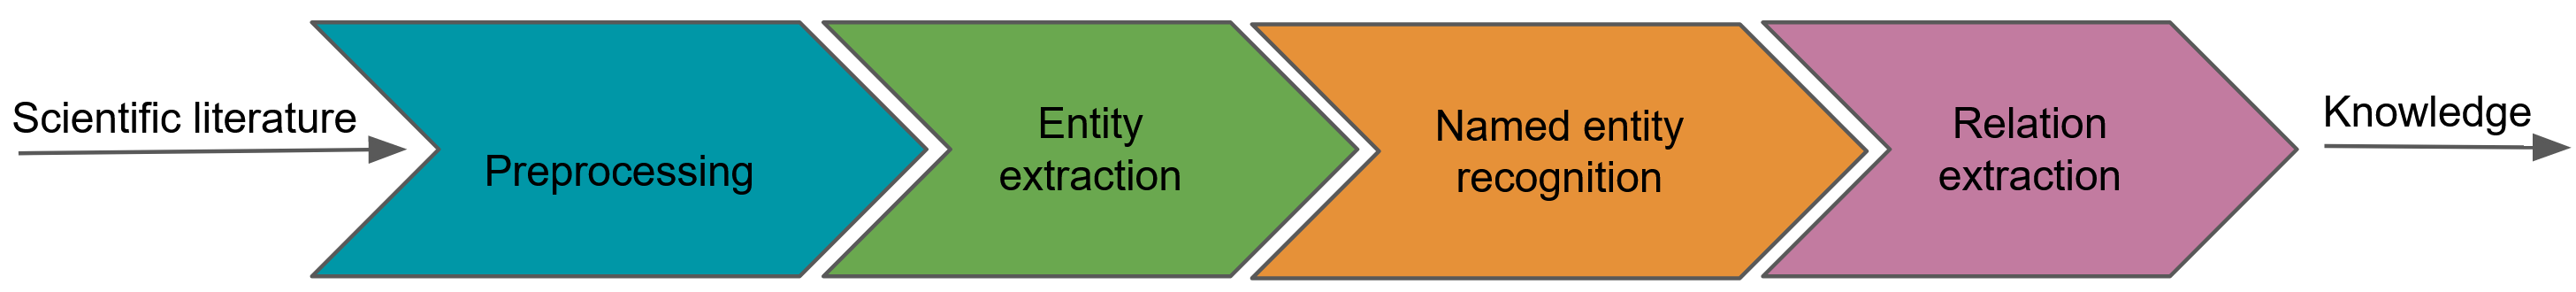
\includegraphics[width=0.9\textwidth]{images/cb_v2.png}
    \caption{Typical knowledge extraction pipeline}
    \label{fig:IE_pipeline}
\end{figure}

\hspace*{3.5mm} Further, the problem of semantic heterogeneity is further compounded due to the flexibility of semi-structured data and various tagging methods applied to documents or unstructured data. Thanks to the SW technologies that offer functionality to connect previously isolated pieces of data and knowledge, associate meaning to them, and represent knowledge extracted from them. In particular, ontology-based named entity relation extraction and disambiguation help unambiguous identification of entities in heterogeneous data and assertion of applicable named relationships that connect these entities together. 


\hspace*{3.5mm} Once instances are extracted, they can be stored as RDF\footnote{Resource Description Framework or RDF is a standard model, the linking structure of a KG forms a directed, labeled graph, where triples are represented in the form of $(u,e,v)$}, where each triple forms a connected component of a sentence for the KG. A number of languages have been proposed for querying a KG in RDF format~\cite{hogan2020knowledge}, including the SPARQL query language for RDF graphs\footnote{SPARQL: \url{https://www.w3.org/TR/sparql11-query/}}, Cypher Query Language\footnote{CypherQL: \url{https://neo4j.com/developer/cypher/}}, Gremlin Query Language\footnote{GremlinQL: \url{https://docs.janusgraph.org/basics/gremlin/}}.
Reasoning over KGs enables consistency checking to recognize conflicting facts, classification by defining taxonomies, and deductive inferencing by revealing implicit knowledge from a set of facts~\cite{futia2020integration}. However, exploration, processing, and analysis of large-scale KGs pose a great challenge to current computational methods. To provide cancer diagnosis reasoning over the DNN models, an integrated domain-specific KG is a mandate, which is further subject to the availability of an efficient NLP-based information extraction method and a domain-specific ontology. %, ML techniques are required. % In a first work, \cite{Zhang.2019} utilized machine learning to find common patterns in flowsheets.
%On the other hand, %development of a KG for cancer genomic requires efficient information extraction and ML techniques. %Additionally, 

\section{Related Work}\label{chapter_8:rw}
%\hspace*{3.5mm} The movement of symbolic AI, also known as Good Old-Fashioned Artificial Intelligence~(GOFAI)~\cite{GoFI}, adopts an opposed paradigm, where the real-world knowledge is not derived by mathematical optimization, but hard-coded in the system exploiting formal languages~\cite{futia2020integration}. Therefore, the system is able to reason on the statements expressed in these formal and logical inference rules. One of the main drawbacks of GOFAI like systems was the their inability of updating knowledge once they were encoded in a rules engine. However, since an expert system is monotonic, adding more rules will enrich more knowledge encoded in the system~\cite{SAI}. Therefore, new rules cannot refresh the old knowledge, as we desire. This is a direct contradiction with basic ML principle in which learning algorithms need to be retrained on new data, which will update the hyperparameters. The updated model preforms better as more updated knowledge will be encoded in the system. The second flaw in SR is that computer itself does not know what the symbols mean~\cite{SAI}, i.e., as they might not be linked to real-world object in a non-symbolic way. This is also a direct contradiction with neural networks as DNNs can link symbols to vectorized representations of the data. Another problem with GOFAI like systems is how to ground symbols and relate them with real-world objects such that it would allow computers to map dynamic real-world objects to symbols and reason about them~\cite{SAI} for better human interpretability. 
This section analyses related works focusing on symbolic and neuro-symbolic reasoning, semantic web technologies, and interactive explanations. Although some of the discussed works are not directly applicable, they still provide the foundations for developing the decision reasoning module for the DSS.

\subsection{Symbolic AI to hybrid AI}
In symbolic AI, an implementation of symbolic reasoning is called rules engine or expert systems that can interact on top of a KB. The symbolic AI paradigm has been a success and could learn flexibly and produce accurate decisions about their inputs. Although a symbolic reasoner can express the interrelations of symbols, a computer does not know what each symbol means, unless we interface it to other representations of the world in a non-symbolic way. One of the main challenges in symbolic AI is how to relate the symbols to other forms of knowledge so that a computer can map the updated or dynamic real-word entities to symbols and reason about them. 
One possible way is to link the symbols into the vectorized representations of the input data, while training a DNN~\cite{SAI,sarker2017explaining}. Although modern DNNs are very powerful at extracting hidden patterns from the input data, making the knowledge acquisition process transparent is open research question in the connectionist community~\cite{futia2020integration}.  
%\subsubsection{Neuro-symbolic reasoning and challenges of current XAI methods}
%They also explained that probabilities are not as important as causal links in order to provide a satisfying explanation. Considering that `black-box' models tend to process data in a quantitative manner, it would be necessary to translate the probabilistic results into qualitative notions containing causal links. Besides, counterfactual explanations can help the user to understand the decision of a model. 
Combining connectionist and symbolic paradigms is a promising way to address this challenge. Symbolic methods are considered less efficient, but they offer several advantageous over connectionist\footnote{Connectionist methods are more precise but opaque and largely resemblance ``black-box'' methods.}~\cite{futia2020integration}:

\begin{itemize}[noitemsep]
    \item It is possible to establish reasoning rules to allow symbolic methods to be constrictive.
    \item The use of a $\mathrm{KB}$ formalized by an ontology allows data processing in a qualitative way.
    \item Being selective is less straightforward for connectionist models than for symbolic ones.
\end{itemize}

%Alejandro et al.~\cite{arrieta2020explainable} outline the trade-off between interpretability and accuracy, i.e., between the simplicity of the information given by the system on its internal functioning, and the exhaustiveness of this description cognitive sciences to create objectively convincing explanations. Explanations are better when constrictive, i.e., a good explanation is not only indicates why the model made a decision $\mathrm{X}$, but also why it made decision $\mathrm{X}$ rather than decision $\mathrm{Y}$. 

%\subsection{Neuro-symbolic AI}
%, albeit it's an old concept. %as DNNs are less flexible and robust to noise compared to DL models. 
\hspace*{3.5mm} In the context of symbolic systems, KGs are a promising solution for the issue of understandability~\cite{futia2020integration}. Biological data and KBs increasingly rely on SW technologies and the use of KGs/KBs for data integration, retrieval, and federated queries~\cite{alshahrani2017neuro}. KGs that interlinked biological entities can be used to provide causal inference, where relationships provide a useful backbone for several reasoning mechanisms ranging from consistency checking~\cite{futia2020integration}. Moreover, KGs and ontologies are natively built to be queried, making them enabled answers to user queries and providing interactive explanations. Ontological reasoning mechanism is often performed by employing a semantic reasoner. A semantic reasoner can provide a symbolic level to interpret the behaviour and the results of a DL model~\cite{futia2020integration}. 

\hspace*{3.5mm} Symbolic AI fuses symbolic and statistical learning theory. However, in a hybrid AI system, knowledge modeling and SW technologies~(e.g., domain ontologies, KBs, and KGs) are combined with a DNN architecture. Research considers introducing semantics into DL paradigm through ontological reasoning a new era towards realization of a hybrid AI system~\cite{futia2020integration}. KGs that are natively built to be explainable\footnote{A DNN model, based on semantic representation of the knowledge, can produce explanations.} can provide the foundation of a semantic layer of a hybrid AI system~\cite{alirezaie2019semantic}. As the symbolic learning paradigm is capable of representing external facts in the form of symbols, hybrid AI systems are appropriate to produce convincing explanations while keeping or improving generic performance. Subsequently, the system enables the user see the explanations that were already deduced based on the embedded knowledge. 

\hspace*{3.5mm} In a recent years, hybrid AI is conceptualize as a neuro-symbolic AI~\cite{futia2020integration}. In a hybrid AI system with necessary human-in-the-loop, a DNN model generates the predictions based on the learned mapping~(i.e., input to output). Predictions are then validated in a weakly supervised manner to identify the wrong predictions. Then, based on existing knowledge from a KB, a semantic reasoner can infer new knowledge to provide more human-interpretable explanations of the queries asked by the user~\cite{futia2020integration}. The benefit is that the model not only learns from the data, but also from explicit and encoded prior knowledge. This learning paradigm not only helps the DNN model to avoid making similar mistakes in successive iterations, but also helps reducing possible prediction biases~\cite{futia2020integration}. 

\hspace*{3.5mm} Giuseppe et al.~\cite{futia2020integration}, identifies three different human-centric challenges in order to develop a hybrid AI system: knowledge matching, cross-disciplinary explanations, and interactive explanations. Seeliger et al.~\cite{seeliger2019semantic} identified matching input features or internal neurons of a DNN model to classes of an ontology or entities of a KG as an important challenge. Sarker et al.~\cite{sarker2017explaining} proposed an approach in which objects within images are mapped to the classes of the suggested ontology. On the basis of classification output of a DNN, a DLx learner is adopted in their approach to create class expressions as a form of explanations. 

\hspace*{3.5mm} Marjan et al.~\cite{alirezaie2019semantic} proposed a new technique called `semantic referee' to improve the performance of a geospatial image classifier. Semantic referee relies on spatial reasoning applied to ontological knowledge to retrieve the error features w.r.t their spatial relations. It is a symbolic-based approach to explain the errors emerged from the classifier and suggesting the corrections. Further, symbolic explanation of the errors is reported to the learning algorithm such that it can avoid making similar mistakes in successive iterations. The classifier consists of a convolutional autoencoder that performs semantic segmentation and classification of geospatial images. Then the semantic referee explains the mistakes made by the classifier based on ontological concepts and feeds it back to the classifier to avoid making the same mistakes~\cite{alirezaie2019semantic}. %However, when it comes with interactive explanations, existing research efforts is rather very limited.

\hspace*{3.5mm} Oltramari et al.~\cite{oltramari2020neuro} has derived a corollary that suggests that `the explainability of AI algorithms is related to how context is processed computationally, based on the machine's perceptual capabilities and on the external knowledge resources that are available'. Such context understanding can only be attained with a neuro-symbolic AI system that is capable of instructing machine perception~\cite{oltramari2020neuro}, i.e., semantics into DNN architectures. %, i.e., knowledge graphs~(KGs)-based reasoning with DNN.
Providing human-level interpretability by ``zooming in'' on individual predictions makes the explanation task easier and trustworthy~\cite{ribeiro2018anchors}. Therefore, to develop and realize a hybrid AI system, interactive explanations is an essential component, rather than static explanations~\cite{futia2020integration}. %However, when it comes with interactive explanations, existing research efforts is rather very limited. 

\hspace*{3.5mm} Sarker et al.~\cite{sarker2017explaining} envision an XAI system for image classification interactively so that human can monitor, fix, and modify decisions based on the explanations. Wang et al.\cite{wang2015explicit} developed an approach based on DNN can extract image contents as KG facts that are interlinked with the DBPedia repository~\cite{lehmann2015dbpedia}\footnote{\url{https://wiki.dbpedia.org/}}. In their system, questions queried by a user are first translated into SPARQL queries that are run over a DBPedia SPARQL endpoint\footnote{\url{https://dbpedia.org/sparql}}. Liao et al.~\cite{liao2018interpretable} proposed a recommender system, which enables user-feedback on human-interpretable domain concepts, where an ontology  provides information~(that are implicitly encoded in the data) to perform inferencing in order to create rules which limit the number of plausible recommendations. 
Although, feature learning methods on graph data are becoming popular, they have not yet widely been applied on structured biological KGs, particularly for cancer genomics. In other ords, apart from these restrictive research initiatives that are mostly suitable for solving research problems concerning images, XAI systems based on neuro-symbolic AI is still not mature. %, especially for cancer genomics. 

\subsection{Knowledge graphs}
Research initiatives are gradually adopting semantic web~(SW) technologies~\cite{karim2018improving} such as knowledge bases~(KBs) and domain-specific ontologies as the means of building structured networks of interconnected knowledge~\cite{futia2020integration}. Hogan et al.~\cite{hogan2020knowledge} has provided a comprehensive review of articles of knowledge graphs, covering knowledge graph creation, enrichment, quality assessment, and refinement. Apart from these literature that focus on the theoretical concepts, several large-scale KGs have been constructed either by manual annotation, crowd-sourcing~(e.g., DBpedia) or by automatic extraction from unstructured data~(e.g., YAGO\footnote{\url{https://github.com/yago-naga/yago3}})~\cite{wang2015explicit} targeting KG analytics for specific use cases. 
%These ontologies are mostly generalized data models that have not yet been used in conjunction with big data to form a KG. 
On the other hand, life sciences is an early adaptor of SW technologies. Numerous research efforts from the scientific communities have focused in constructing large-scale KGs for the life science research. For example, Bio2RDF\footnote{\url{https://github.com/MaastrichtU-IDS/bio2rdf} and PubMed knowledge graph~\cite{xu2020building}} are developed to accelerate the bioinformatics research. The former integrates 35 life sciences datasets such as dbSNP, GenAge, GenDR, LSR, OrphaNet, PubMed, SIDER, WormBase, contributing 11 billion RDF triples. 

\hspace*{3.5mm} Alshahrani et al.~\cite{alshahrani2017neuro}, built a biological KG  based the gene ontology~(GO), human phenotype ontology~(HPO), and disease ontology. Then, they performed feature learning over the KG. Their method combines knowledge representation using symbolic logic and automated reasoning, with neural networks to generate embeddings of nodes. Then the learned embeddings are used in downstream application development such as link prediction, finding candidate genes of diseases, protein-protein interactions, and drug target relation prediction. Hasan et al.~\cite{hasan2020knowledge} developed a prototype KG based on the Louisiana Tumor Registry dataset\footnote{https://sph.lsuhsc.edu/louisiana-tumor-registry/}. Their approach provides scenario-specific querying, schema evolution for iterative analysis, and data visualization. Although, found to be effective at population-level treatment sequences, being built on a limited data setting, their KG does not provide comprehensive knowledge about cancer genomics for the majority of the cancer types.

\hspace*{3.5mm} Hu et al.~\cite{hu2015semantic} developed a breast cancer KG. The KG is developed by integrating: i) Dutch medical guidelines of breast cancer\footnote{A semantic representation of evidence-based medical guidelines from Dutch medical guidelines} that contain conclusions, their evidences, and the semantic annotations of the conclusion with medical terminologies like UMLS and SNOMED CT, ii) genomic data of female patients of breast cancer, iii) clinical trials of breast cancer from the official NCT website, iv) semantic annotations of the eligibility criteria of clinical trials of breast cancer that are generated XMedLan\footnote{A Xerox natural language processing tool for medical text}, iv) selected medical publications of breast cancer from the PubMed data set released by the Linked Life Data\footnote{A semantic data integration platform for biomedical domain}. 
Although, these KGs can be used to explore the relationship among various knowledge and data sources of breast cancer and support for clinical DSS, there are no comprehensive KBs or KGs have been developed targeting wide variety of cancer types. 
%\subsection{Interactive explanations}
\subsection{Structured knowledge  extraction}
In biomedical treatment protocol, structured data is first extracted from various unstructured sources such as pathology reports, radiology reports, and medical records, before storing in a database for reporting and diagnosis purposes. In hospital information system or electronics health records, cancer registry data is typically categorize each reported cancer case or tumor at the time of diagnosis~\cite{hasan2020knowledge}. Besides, it may contain demographic information about the patient such as age, gender, location at time of diagnosis, planned and completed primary treatment information, and survival outcomes~\cite{hasan2020knowledge}. Besides, cancer-related scientific articles that reports unstructured data also provide facts and knowledge about cancer characteristics, treatments, and outcomes. Although, extract information from structured data is easy, extracting the same from unstructured data is highly domain specific. 

\hspace*{3.5mm} Apart from the oncogenes and protein-coding genes, proto-oncogenes are a group of genes that cause normal cells to become cancerous when they are mutated~\cite{slamon1987proto}. An important difference between oncogenes and a POSTF is that oncogenes result from the activation of proto-oncogenes, whereas a POSTF itself cause cancer when they are inactivated. Mutations in proto-oncogenes are typically dominant in nature, and the mutated version of a proto-oncogene is called an oncogene~\cite{slamon1987proto}. For example, abnormalities of the TP53 gene have been found in more than half of human cancers\footnote{Source: \url{https://www.cancer.org/cancer/cancer-causes/genetics/genes-and-cancer/oncogenes-tumor-suppressor-genes.html}}. \hspace*{3.5mm} Shen et al.~\cite{POSTF} have reported that some genes have both oncogenic and tumor-suppressor functionality called proto-oncogenes with tumor-suppressor function~(POTSF). Majority POTSF genes act as transcription factors or kinases and exhibit dual biological functions, e.g., they both positively and negatively regulate transcription in cancer patient cells~\cite{POSTF}. Besides, some specific cancer types such as leukemia are over-represented by POTSF genes, whereas some common cancer types like lung cancer are under-represented by them~\cite{POSTF}. 

\hspace*{3.5mm} Since both structured and unstructured cancer data is constantly expanding and evolving, linking a large volume of heterogeneous data sources is quite challenging, as heterogeneous data sources often do not follow any common data-storing standard~\cite{hasan2020knowledge}. Feature- or kernel-based methods such as the conditional random field~(CRF) are earlier approaches used for the NER and relation extraction in a pipeline setting~\cite{xue2019fine}. However, performance of the traditional approaches heavily depends on manual feature engineering, domain-specific knowledge, and a deep understanding of linguistics~\cite{xue2019fine}. Therefore, approaches based on DNNs have emerged that are not only capable of automatic extraction of structured knowledge, but also leverage end-to-end learning capability~\cite{dogan2019fine}. Lately, several deep architectures based on recurrent types neural networks have been proposed for entity recognition and relation extraction. 

\hspace*{3.5mm} Approaches based on Bidirectional Long Short Term Memory~(Bi-LSTM) or Gated Recurrent Unit cells are more widely used~\cite{zheng2017joint}. For example, Geng et al.~\cite{zhang2020semi} used a Bi-LSTM network with a subsequent CRF, where inputs to the Bi-LSTM are concatenated word representations that combine pre-trained contextual word embeddings using embeddings from language models~(ELMo)~\cite{peters2018deep}, character-level word representations, and positional features of the word in the document. Joint entity and relation extraction approaches are also proposed. Zhang et al.~\cite{zheng2017joint} used joint-BiLSTM -a joint tagging method that can transform both tasks into sequence tagging through parameter sharing in an end-to-end learning setting. Although Bi-LSTM approaches outperform CRF-based approaches, their shortcoming lies in the incapability of semantic annotation and validation of the extracted entities and relations, i.e., not all relations can be represented by triggered words~\cite{sun2020biomedical}. 
On the other hand, transformer language models have become the de-facto standard for representation learning in NLP, as it is feasible to perform domain-specific fine-tuning in a transfer learning setting. Compared to transformer models that benefit from abundant knowledge from pre-training and strong feature extraction capability, approaches based on Bi-LSTM have a lower generalization performance~\cite{xue2019fine}. 

\hspace*{3.5mm} Bidirectional Encoder Representations from Transformers~(BERT)~\cite{devlin2018bert} is a language model that utilizes bidirectional attention mechanism and large-scale unsupervised corpora to obtain effective context-sensitive representations of words in a sentence~\cite{xue2019fine}. Subsequently, several variants of BERT are proposed and widely used as transformer language models for a variety of downstream NLP tasks like NER. Sun et al.~\cite{sun2020biomedical} employed transformer for predicting entity labels, where word representations are obtained from a pre-trained BERT model. BERT-based approaches have also been applied to scientific texts~(e.g, SciBERT~\cite{Beltagy2019SciBERT}) and adapted in other domain such as ChemBERTa~\cite{chithrananda2020chemberta} in chemical engineering for molecular property prediction.
%\hspace*{3.5mm} The majority of traditional IE approaches are focused on informal text~(e.g., social media texts), or on biomedical text, while only a little literature on CE related text exists~(e.g. PubMedInfo Crawler~\cite{kanwal2019pubmedinfo}, chemical patents~\cite{sun2020biomedical}). In particular, very little attention is paid to IE for chemical process design. 
Xu et al.~\cite{xu2020building} have shown that bio-entity extraction based on BioBERT~\cite{lee2020biobert} can significantly outperform DNN-based methods. As the transformer-based language models have a great potential for all the tasks involved in information extraction, approaches that combine NLP, information retrieval, and SW technologies can be more effective for extracting knowledge from unstructured texts with high accuracy~\cite{anantharangachar2013ontology}. %Due to the variety of underlying ontologies and relation types, relation extraction task is highly domain specific. 
In other words, an ontology-guided information extraction method needs to be combined with state-of-the-art transformer language models. % for extracting and presenting information from both structured and unstructured data sources. 

\section{Methods}\label{chapter_8:mm}
%\hspace*{3.5mm} Since cross-disciplinary explanations are the mandate for accurate diagnosis of cancer, querying the KG and providing interactive explanations about learned biomarkers is the focus of this chapter. In the end, a domain-specific KG is developed as the basis of the KB by reusing concepts and knowledge from the several existing ontologies and KBs, containing domain knowledge, vocabulary, facts, and rules about human diseases, annotations about genes, and evidence from scientific literature. That is, knowledge, facts, and data from heterogeneous sources such as scientific articles, ontologies and KBs are integrated in the KG. The KG forms the foundation of a semantic layer, which is used to `harmonize' metadata schema and vocabularies.
%\hspace*{3.5mm} A domain-specific KG is an explicit conceptualization of a KG to a specific subject-matter domain represented in terms of semantically interrelated entities and relations~\cite{abu2020domain}. Building a domain-specific KG has several core requirements: i) formal conceptualization to indicate the logical design of the KG depicted by a specific, predefined domain-specific ontology; ii) modeling of domain knowledge, represented by semantically interrelated entities and relations~\cite{abu2020domain}. 
%This chapter shows how SW technologies can help build a domain-specific KG. 
Since a semantic reasoner infers and produces new knowledge from existing knowledge to answer interactive queries, this thesis hypothesize\footnote{\textbf{H5}: Based on a set of axioms and explicit facts, ontological reasoning can characterize diagnosis decision by inferring implicit but known facts} that ontological reasoning can infer new knowledge from existing knowledge and DLx axioms. In other words, based on a set of axioms and explicit facts, a semantic reasoner will able to derive implicit, but previously known facts from a KG. %Subsequently, a semantic reasoner would be able to gap between current approach and the expectation by providing automated reasoning. Thus, a hybrid AI by combining semantic reasoning and a DNN has the full potential to realize and build an XAI system capable of providing the reasoning in the clinical setting. 
The benefit would lie on the fact that the model learns not only from the data but also from explicitly encoded and prior knowledge from the ontology and avoids making similar mistakes in successive iterations. %We are one of the first batch of researchers to develop a symbolic AI for the clinical diagnosis decision system. 

\hspace*{3.5mm} In this section, we discuss the approach for decision reasoning in detail. The workflow of the overall reasoning method shown in \cref{fig:reasoning_wf} is inspired by an hybrid AI system proposed by Giuseppe et al.~\cite{futia2020integration} and the `Semantic Referee' proposed by Alirezaie et al.~\cite{alirezaie2019semantic}. Further, our approach utilizes the previously generated decision rules. We developed an ontology which can enable semantic reasoning for verification of the predictions for relations between diseases and genes. The ontology we introduce here allows the aforementioned reasoning by using different rules which are derived from the ontology itself. Subsequently, the SR would help inferred and validate the matched concepts, enrich with domain knowledge and returns the modified rules before explaining to end users, where the query and reasoning mechanisms over KGs enable interactive and rule-based explanations. 

\begin{sidewaysfigure}
	\centering
	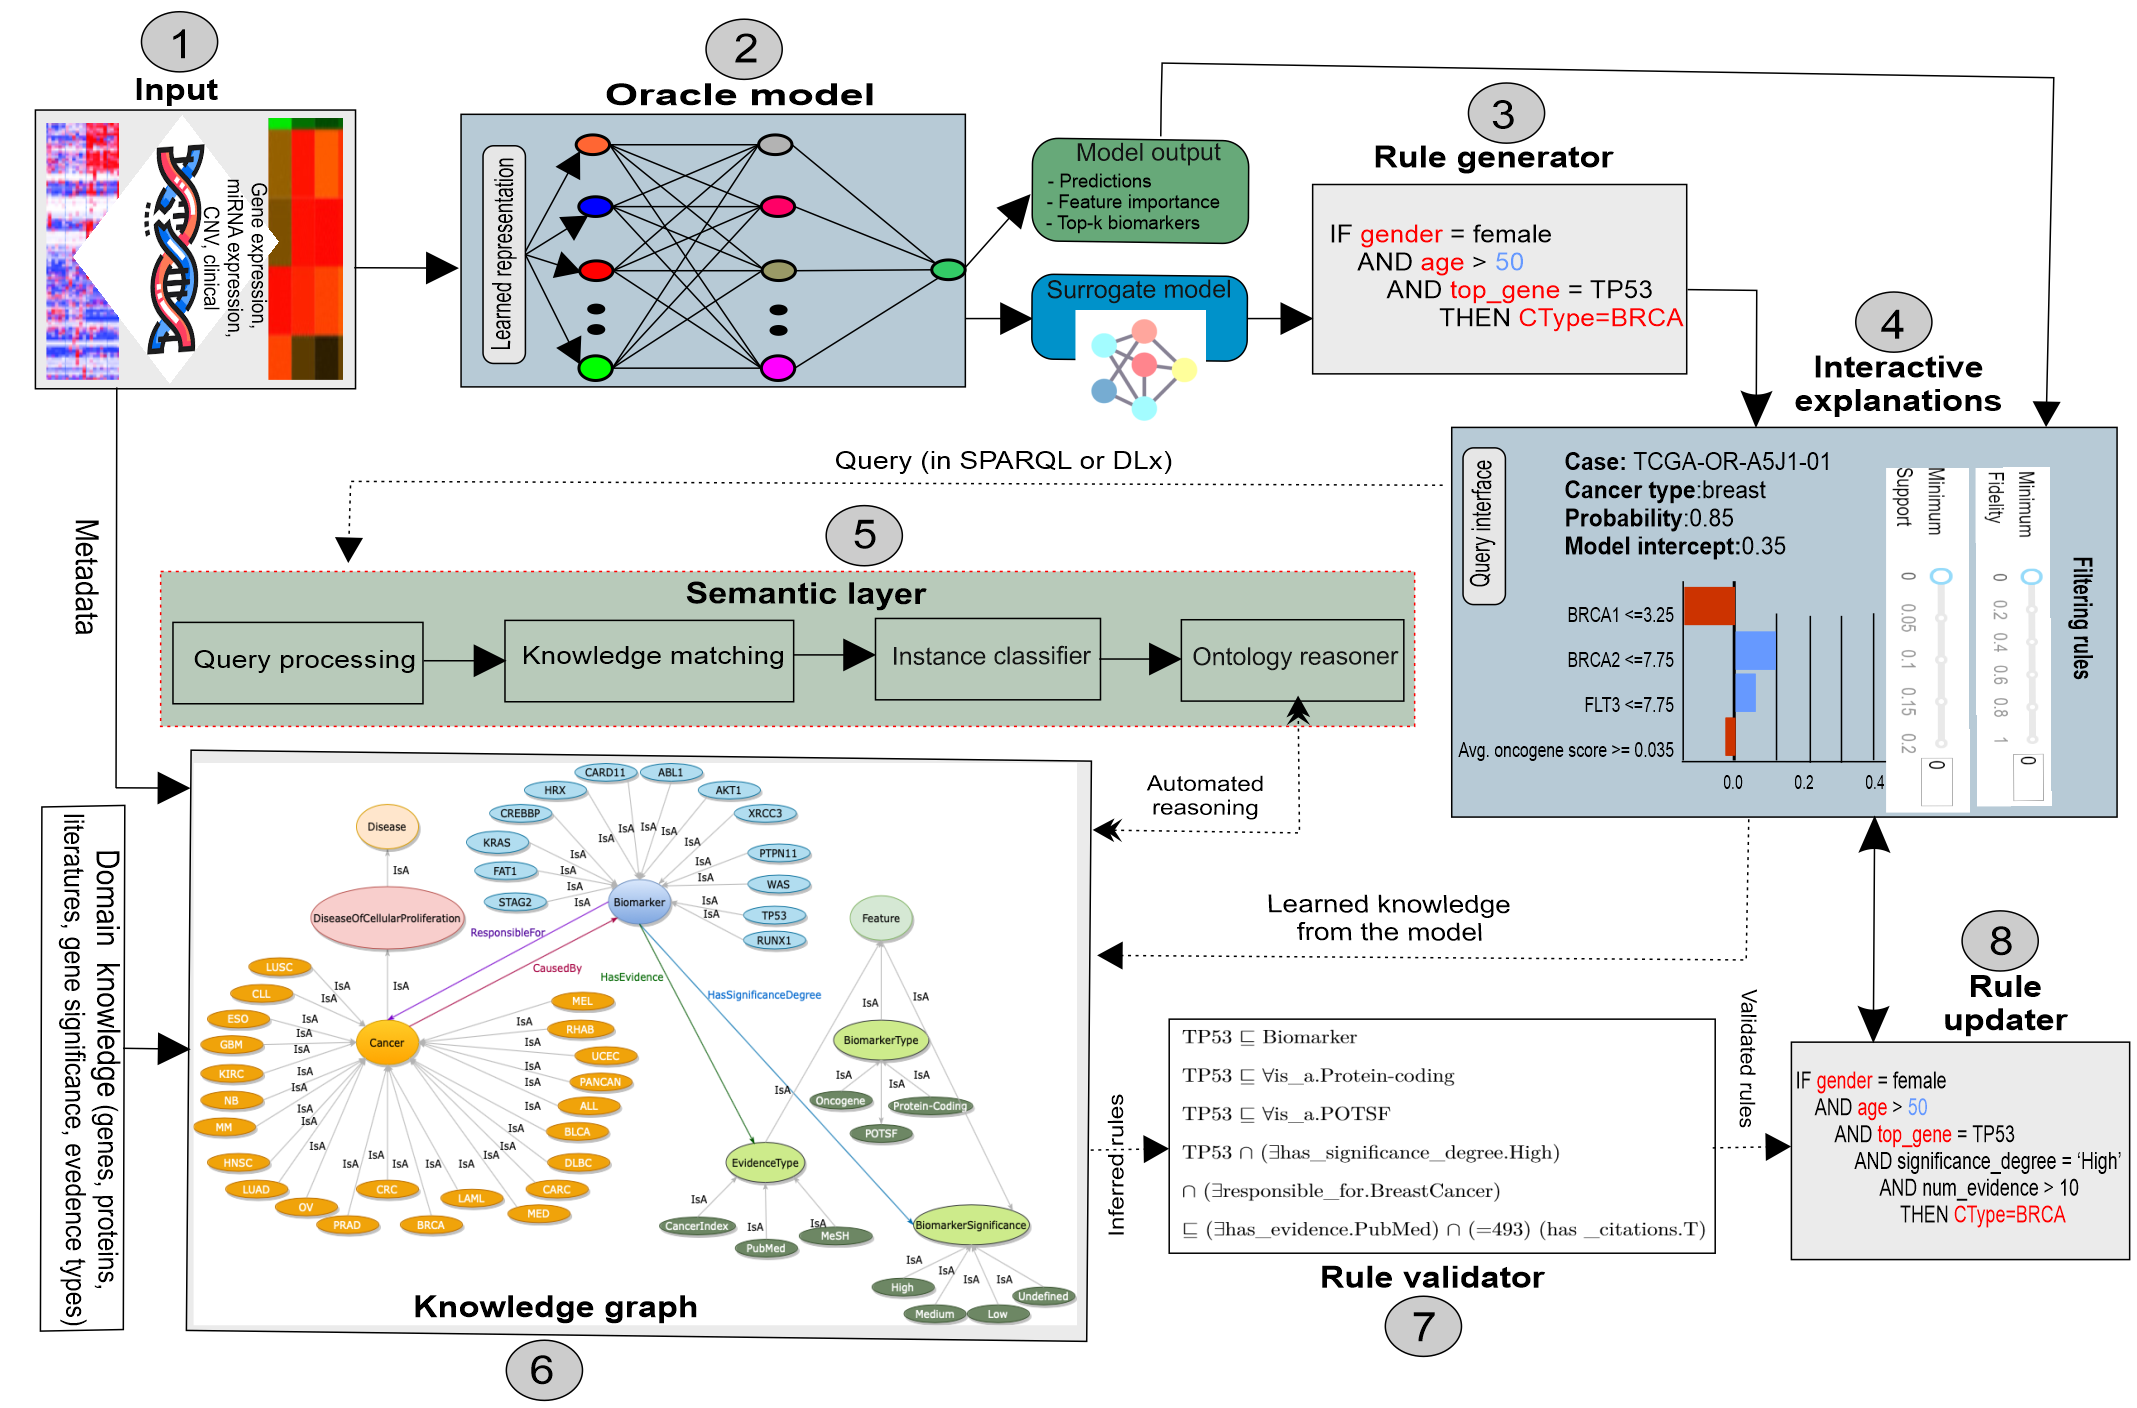
\includegraphics[scale=0.9]{images/reasoning_wf.png}
	\caption{Workflow of the overall reasoning method} 
	\label{fig:reasoning_wf}
	\vspace{-2mm}
\end{sidewaysfigure} 

\hspace*{3.5mm} Since cross-disciplinary explanations are the mandate for accurate diagnosis of cancer, querying the KG and providing interactive explanations about learned biomarkers is the focus of this chapter. In a nutshell, a semantic reasoner provides the foundation of the semantic layer, where a reasoner infers and produces new knowledge from existing knowledge from the KB in order to answer interactive queries. 
%\subsection{Problem statement}
%However, to know the global-behaviour and validation of the generated decision rule set,
The goal to acquire knowledge and store it in KB is to provide querying facilities for the end-user in interactive explanation scenario. In a similar, argument, the main reasoning task is query answering. However, in our case the querying is enriched by a rule-based layer. Thus the reasoner takes into account the domain-knowledge represented within the rules while querying. 

\subsection{Problem statement}
Given a decision rule set $R$, the problem is to perform ontological reasoning for each antecedent $a$. The knowledge matching module performs matching antecedents $F$ with the ontological concepts by applying ontology-based axioms classification in the form of DLx format. %Ontological relations in the form of logic-based axioms are used by reasoning methods to infer both implicit and explicit information~\cite{alirezaie2017ontology}. 
Then from a set of facts $\mathcal{F}$ and a set of rules $\mathcal{R}$, i.e., all the deducible knowledge are computed until no rule is applicable. If the closure of a set of facts $\mathcal{F}$ is the same as $\mathcal{F},$ i.e., $\mathrm{Cl}_{\mathcal{R}}(\mathcal{F})=\mathcal{F}$, then we say that $\mathcal{F}$ is closed under the rules or deductively closed~\cite{garoufallou2016metadata}. We hypothesize that a query $Q$\footnote{A query in human language, a SPARQL, or query in DLx format} has an answer within a knowledge base $\mathcal{K}$ if and only if $\mathrm{Cl}_{\mathcal{R}}(\mathcal{F}) \models Q$, where $\models$ refers to the usual first-order entailment~\cite{garoufallou2016metadata}. 

\subsection{Construction of the knowledge graph}
Depending on the hierarchy of abstraction, relations between concepts can be more complicated, making it difficult to interpret. However, based on existing concepts, an ontology-based reasoning process is able to retrieve  domain-specific concepts using the subsumption relations between concepts~\cite{alirezaie2019semantic}. Since a rule set satisfying a certain threshold of minimum support and fidelity are already generated, they already can be reused to provide interactive explanations. However, to provide additional interpretations about a concept, a semantic layer is constructed. The KG forms the foundation of a semantic layer, which is used to `harmonize' metadata schema and vocabularies.

\hspace*{3.5mm} The semantic layer consists of query processing module, knowledge matching module, instance classifier, and the ontology reasoner. This layer provides an interface between the KG and the rule generator. Since a domain-specific ontology is a mandate, a domain-specific ontology is developed in which a set of vocabulary and facts we will embed into. Subsequently, the ontology is modelled as a KG by additional properties about the concepts. Eventually, the ontology containing domain-specific knowledge and facts about cancer genomics is composed of the following three main components:

\vspace{-2mm}
\begin{itemize}[noitemsep]
    \item \textbf{Vocabulary} - containing knowledge about concepts and relations w.r.t cancer genomics. 
    \item \textbf{Rules} - representing rules~(we treat it the rule-base) that encode generic knowledge. 
    \item \textbf{Facts} - containing factual knowledge about cancer genomics subjects.
    \vspace{-4mm}
\end{itemize}

\subsubsection{Integrated ontology development}
Ontologies classify things and define more specific relations and attributes, where entities can be specifically classified and thus become an instance of one or more classes. In conjunction, restrictions can now be expressed in order to develop a more consistent knowledge model. Ontologies are also used to take advantage of inference mechanisms. Since the semantic annotations are typically based on predefined concepts w.r.t. biological entities, a domain-specific ontology is required to perform ontological reasoning. Annotations also help enrich the KG with domain knowledge about relations between concepts to facilitate more complex and elaborate reasoning. 

\begin{figure*}
	\centering
	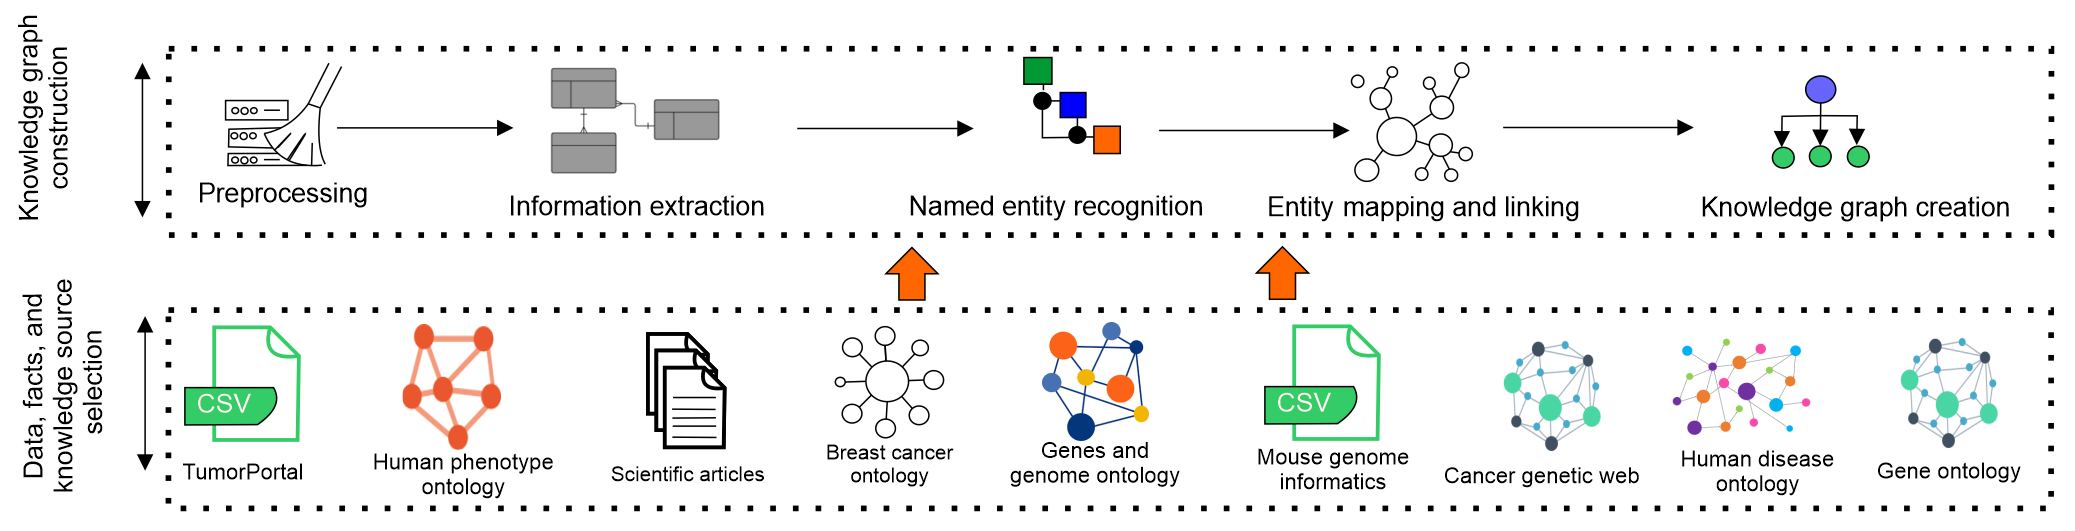
\includegraphics[scale=0.7]{images/KG_construction_steps.png}
	\caption{Workflow of the overall knowledge graph construction} 
	\label{fig:kg_creation}
	\vspace{-2mm}
\end{figure*} 

\hspace*{3.5mm} The main components of an ontology are individuals~(instances or objects) of classes~(distinct types of concepts exist in the data), relationships~(ways to relate classes and individuals), and attributes~(aspects, properties, features, characteristics that objects and classes can have). Building a domain-specific KG has several core requirements: i) formal conceptualization to indicate the logical design of the KG depicted by a specific, predefined domain-specific ontology, ii) modeling of domain knowledge, represented by semantically interrelated entities and relations~\cite{abu2020domain}. %, which will be used to perform the 
In our approach, instead of building a new ontology from scratch\footnote{Part of the ontology was developed by Lina Teresa Molinas Comet \& Suchanda Bhattacharyya as part of HiWi job}, we build it in the form of KG based on several existing ontologies. We reuse existing and rich ontologies to represent domain knowledge about human diseases, annotations about genes, cancers, mutations, metadata ~(i.e., labels and provenance), and corresponding evidences from scientific literature. 
\subsubsection{Ontology modelling}
As a ground basis, we used the ontology of gene ontology~(GO), human phenotype ontology, disease ontology, genes and genomes~(OGG)\footnote{\url{https://bioportal.bioontology.org/ontologies/OGG/?p=classes&conceptid=root}}, and the human disease ontology~(DOID)\footnote{\url{https://bioportal.bioontology.org/ontologies/DOID/?p=classes&conceptid=root}}. Our decision was made based on the fact that those two ontologies model entities about genes and genomes, and human diseases respectively. We inherited the metadata of the entities from both ontologies. Additionally, we complemented the metadata for the entities by adding information from two other resources, i.e., TumorPortal\footnote{\url{http://www.tumorportal.org}} and the cancer genetics website\footnote{\url{http://www.cancer-genetics.org/genes_a.htm}}. 

\hspace*{3.5mm} As shown in \cref{fig:kg_creation}, we reused semantic concepts from several sources to model our ontology, which can reflect the structural aspects of the connection between biomarkers~(e.g. oncogenes, protein-coding) and cancer types~(e.g. breast cancer, colorectal cancer). We aim it using this ontology for inferring rules which can be used as a reasoning engine towards simple querying to get domain-specific information about a biomarker responsible for certain cancer types. Moreover, the types of queries that can be answered based on the ontology reasoner are also extended to the evidence supporting a specific relation, as well as the degree of significance of a gene for certain cancer types. 

\paragraph{Human disease ontology:} \hspace*{-2.5mm} as an initial resource we used the DOID, which provides a general schema describing human related diseases. The DOID has been developed by `BioPortal', which provides a comprehensive hierarchical controlled vocabulary for human disease representation, in biomedical resources, health, human, neurologic disease, and neurological disorder categories. The ontology is organized in classes and sub-classes, where the most general class is \texttt{doid:Disease}, which contains different subclasses for each general group of diseases which in turn contain other specific sub-classes like diseases. The relation between entities are expressed with different axioms. 

\hspace*{3.5mm} The whole structure of the DOID ontology is not inherited since it contains many sub-groupings that are not crucial for our requirement. Instead, we focused on the sub-classes `disease of cellular proliferation' and `disease of anatomical entity', and more specifically in the classes containing `cancer' related facts about cancer types. \Cref{fig:oncoontology14} shows the hierarchical relation between between classes and sub-classes. \\ 

\vspace{-4mm}
{\scriptsize 
    \hspace{-1mm} doid:Disease$\sqsubseteq$owl:Thing \\
    \hspace{2mm} doid:DiseaseOfCellularProliferation$\sqsubseteq$ doid:Disease\\
    \hspace{2mm} doid:Cancer$\sqsubseteq$ doid:DiseaseOfCellularProliferation\\
    \hspace{2mm} doid:DiseaseOfAnatomicalEntity$\sqsubseteq$ doid:Disease\\ 
    \hspace{2mm} doid:BreastCancer$\sqsubseteq$doid:BreastDisease$\sqsubseteq$doid:ThoracicDisease$  \sqsubseteq$doid:DiseaseOfAnatomicalEntity.} \\

\vspace{-4mm}

\begin{figure*}
	\centering
	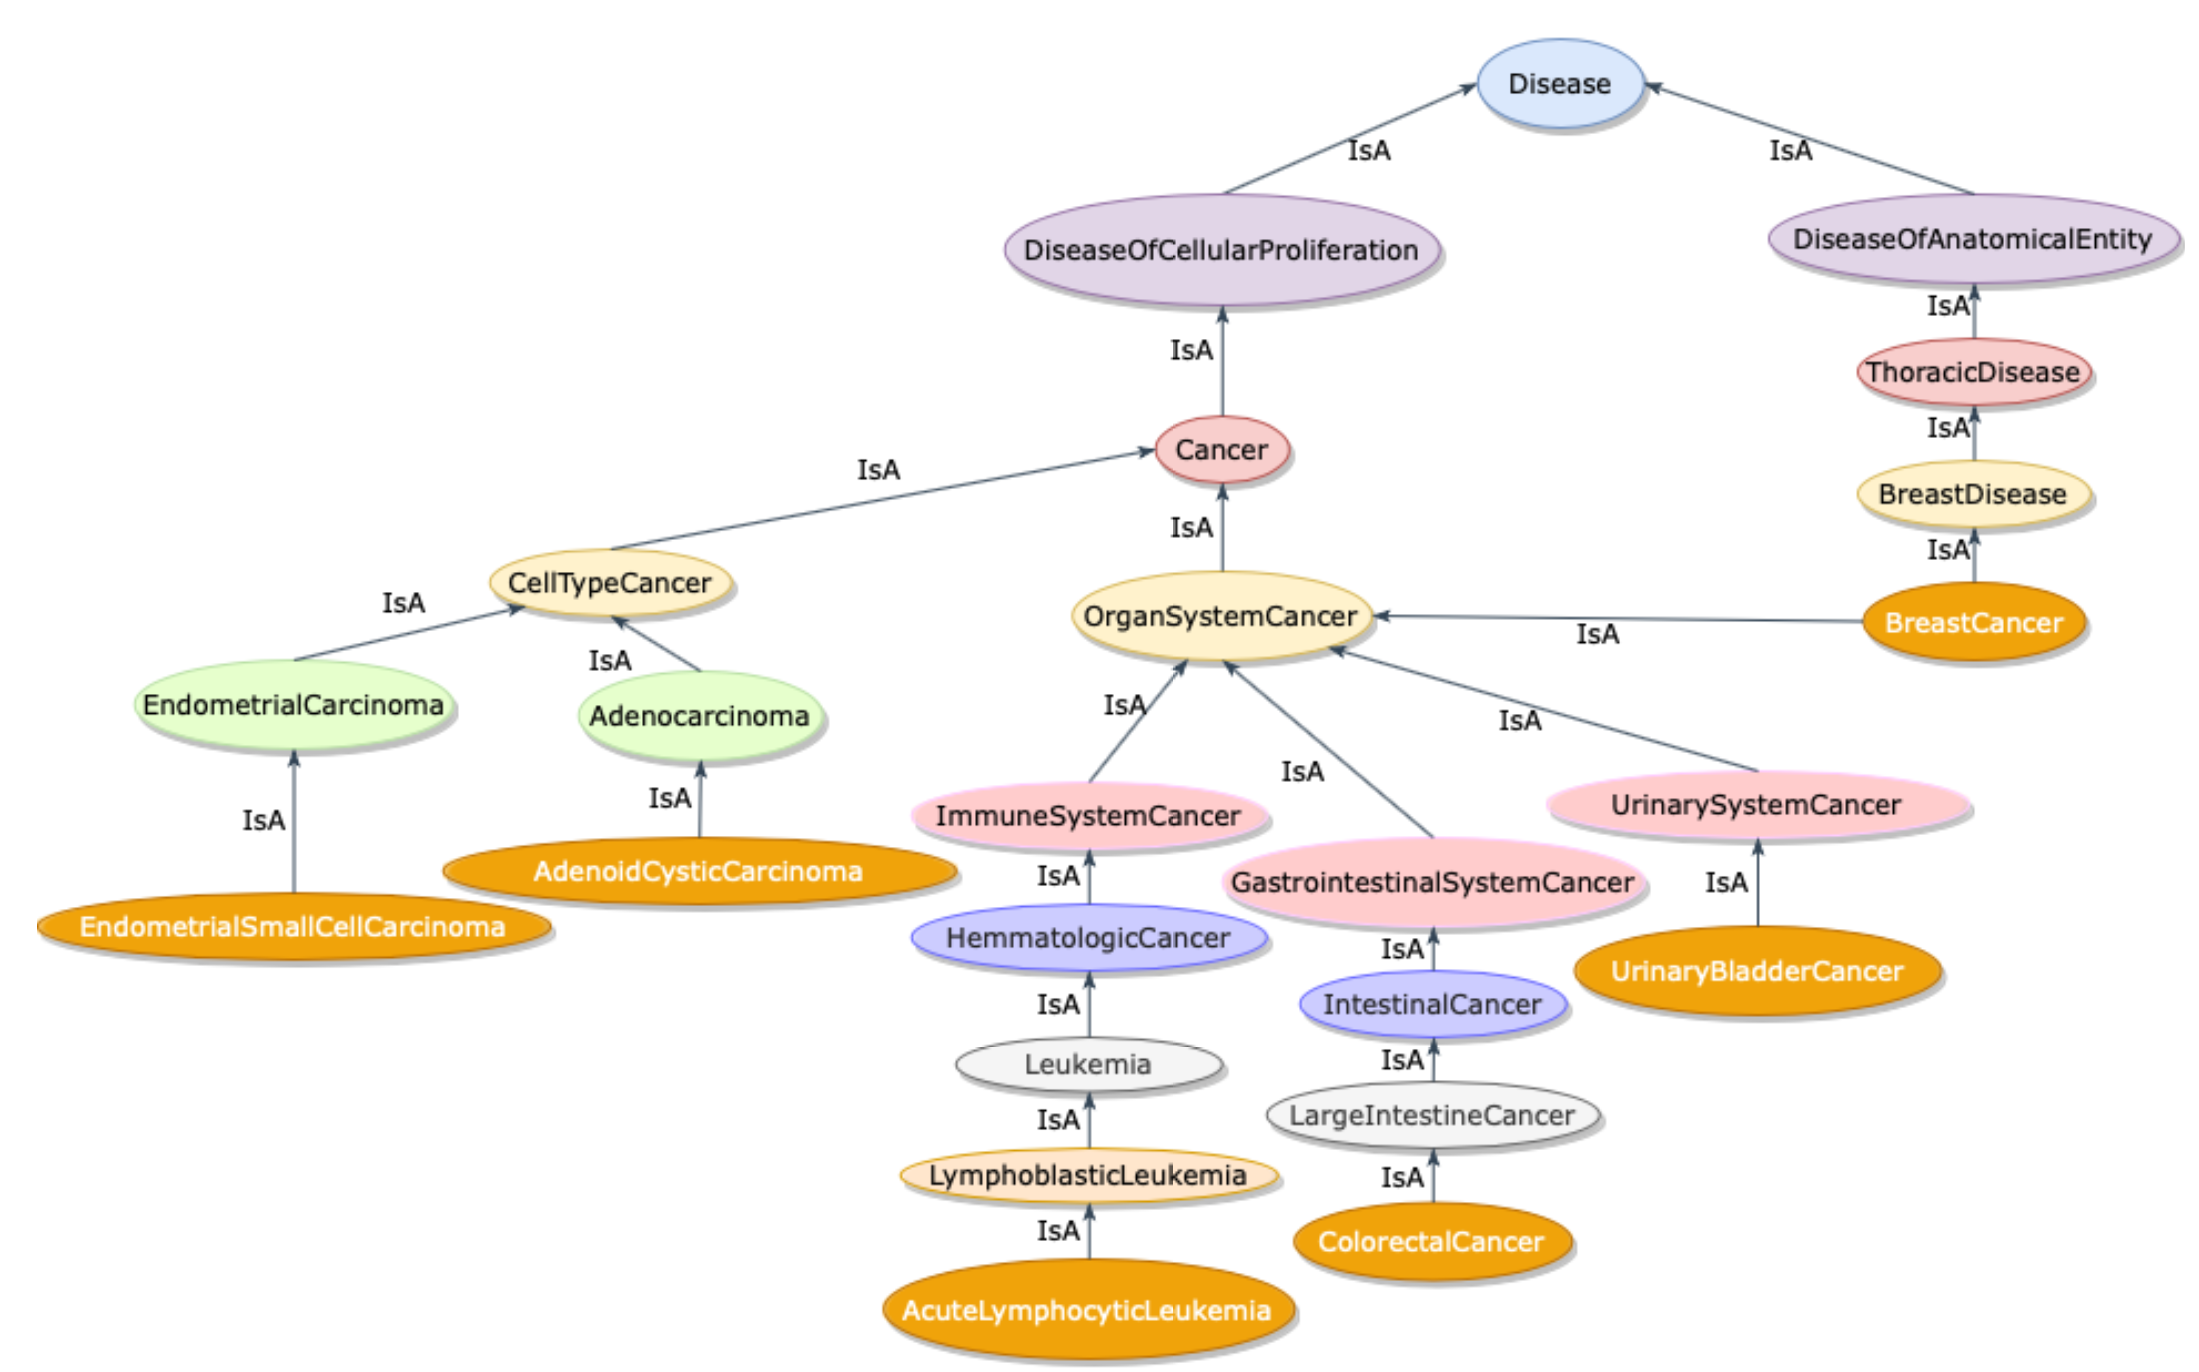
\includegraphics[scale=0.5]{images/do.png}
	\caption{High-level view of some part of the DOID ontology} 
	\label{fig:oncoontology14}
	\vspace{-2mm}
\end{figure*}

\hspace*{3.5mm} Each class in the DOID ontology is described with annotations indicating different properties of that object. For example, the annotation `prefLabel' indicates the name of the object, but in addition the annotation `has\_exact\_synonym' indicates the other names with which that object is known in other ontologies. We inherited all the object properties of the entities, namely cancer types.

\paragraph{Ontology of genes and genomes:} \hspace*{-2.5mm} to map diseases with the responsible genes associated with, we used the OGG in which we model the properties of the biomarkers. The OGG ontology uses a hierarchical structure similar to the DOID ontology. However, we focus on the entities under the class `gene of Homo sapiens' which describe genes that are present in humans. It is important to mention that we just inherited the annotations of the properties for each biomarkers~(e.g., gene), such that the gene properties related to certain cancer types were only extracted. \Cref{fig:ogg_ontology} shows the hierarchical relation between classes and sub-classes.\\

\vspace{-4mm}
{\scriptsize
    \hspace{-1mm} \noindent ogg:DiseaseOfCellularProliferation $\sqsubseteq$ doid:Disease\\
    \hspace{2mm} ogg:Cancer$\sqsubseteq$doid:DiseaseOfCellularProliferation\\
    \hspace{2mm} doid:DiseaseOfAnatomicalEntity$\sqsubseteq$doid:Disease\\
    \hspace{2mm} ogg:BRCA1$\sqsubseteq$ogg:ProteinCodingGeneOfHomoSapiens$\sqsubseteq$ogg:GeneOfHomoSapiens$\sqsubseteq$ ogg:Gene$\sqsubseteq$ogg:MaterialEntity$\sqsubseteq$ ogg:Entity.}\\

\vspace{-2mm}
\begin{figure*}
	\centering
	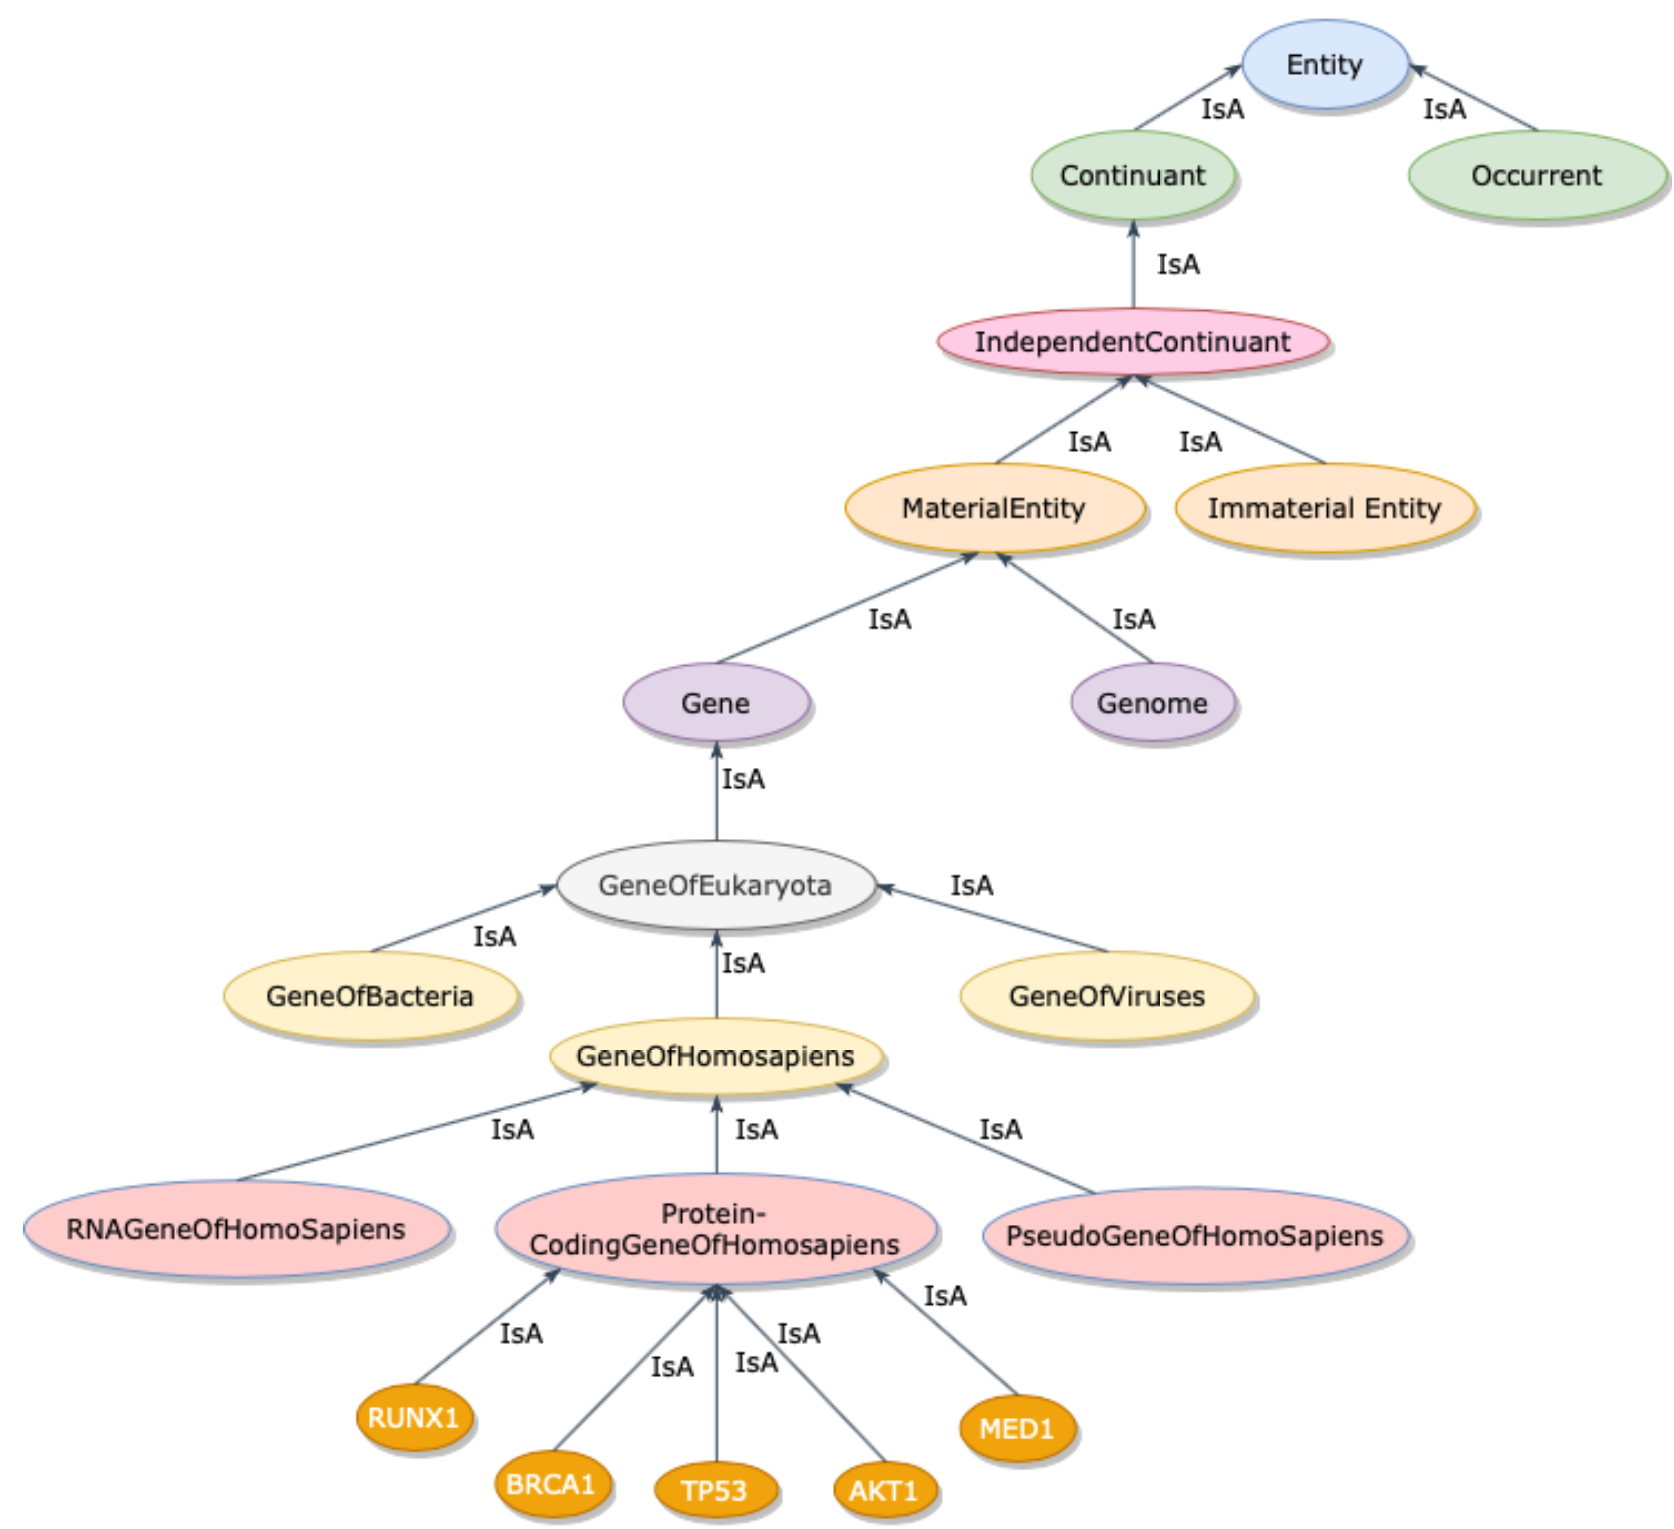
\includegraphics[scale=0.5]{images/go.png}
	\caption{Partial high-level view of the OGG ontology} 
	\label{fig:ogg_ontology}
	\vspace{-2mm}
\end{figure*}

\vspace{-2mm}
\hspace*{3.5mm} Each entity and class is annotated with properties ranging from the name of the entity `preferred name', to the definition, and the alternatives terms `alternative term' used to identify a particular entity. We inherited all the properties for each entity in our new ontology.

\begin{figure*}[h]
	\centering
	\begin{subfigure}{0.48\linewidth}
	\centering
		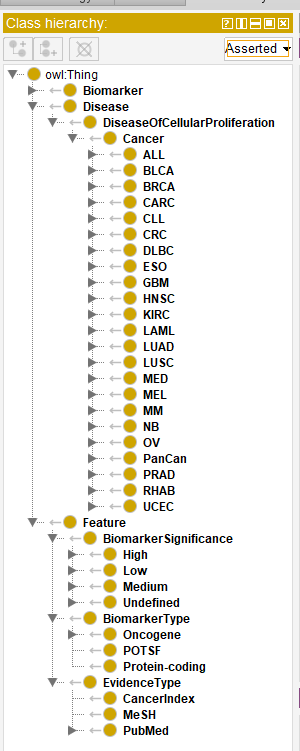
\includegraphics[width=0.55\linewidth,height=70mm]{images/OncoReferee.png}
		\caption{High-level view of the ontology}
        \label{fig:main_ontology_pro_view}
	\end{subfigure}
	\begin{subfigure}{0.48\linewidth}
		\centering
		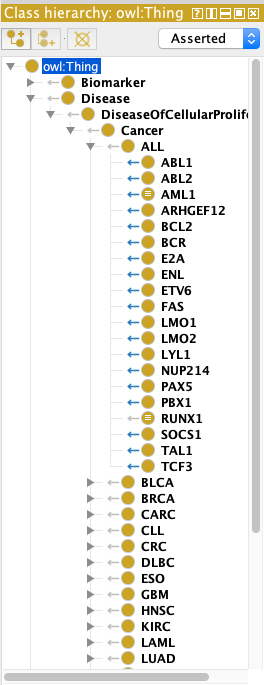
\includegraphics[width=0.55\linewidth,height=70mm]{images/biomarker_view_2.png}
		\caption{Properties of an entity in the disease class}
        \label{fig:diseases_class}
	\end{subfigure}
	\begin{subfigure}{.48\linewidth}
		\centering
		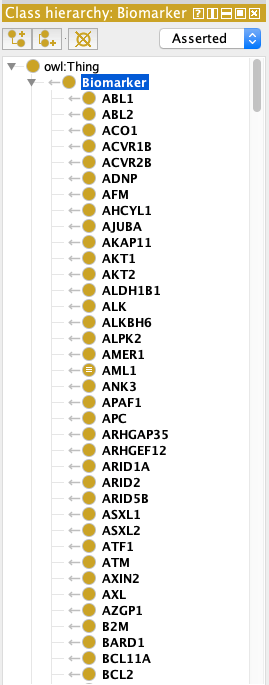
\includegraphics[width=0.55\linewidth,height=70mm]{images/biomarker_view.png}
		\caption{Biomarker class for different cancer types}
        \label{fig:annotations_for_genes}
	\end{subfigure}
	\iffalse
	\begin{subfigure}{0.48\linewidth}
		\centering
		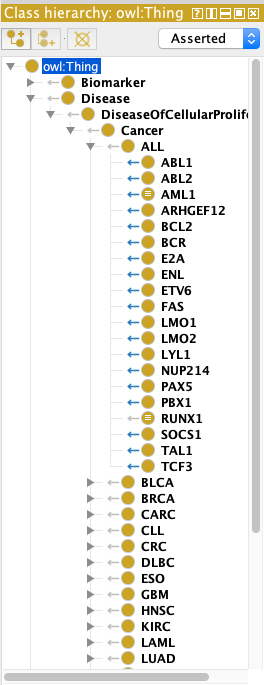
\includegraphics[width=0.55\linewidth,height=70mm]{images/biomarker_view_2.png}
		\caption{Disease subclasses to corresponding cancer types}
        \label{fig:diseases_sub_class}
	\end{subfigure}
	\fi 
	\caption{Hierarchical view of the biomarker and disease class} 
	\label{fig:property_enrich_annotations_for_genes}
	\vspace{-4mm}
\end{figure*}

\paragraph{Disease ontology, breast cancer ontology, and cancer genetics web} \hspace*{-2.5mm} - the disease ontology~(DO) is a standardized ontology for human disease, which aims to provide consistent, reusable and sustainable descriptions of human disease terms, phenotype characteristics, and medical vocabulary disease concepts. DO semantically integrates disease and medical vocabularies via cross mapping of DO terms from MeSH, ICD, NCI, SNOMED, and OMIM. The BCO from EBI provides the domain knowledge about breast cancer, which is also a good source of carcinogenics to understand the relations of different biological entities for breast and other cancer. Further, DO provides an integrated information from several data source and analysis of the literature using data from PubMed and CancerIndex.org. Further, it also provides and integrated view of the latest research abstracts relating to genes, proteins and cancer.  

\hspace*{3.5mm} Our decision was made based on the fact that those two ontologies model entities about genes and genomes, and human diseases respectively. We inherited the metadata of the entities from both ontologies. Besides we enriched our ontology with knowledge from mouse genome informatics~(MGI) that provides genomic data to study human disease, while the TumourPortal provides annotations about genes, cancers, and DNA mutation. Additionally, we complemented the metadata for the entities by adding information from two other resources, namely the TumorPortal and the cancer genetics website. We also integrated knowledge from Tumor Portal website from which we took information regarding the significance degree of the genes which are significantly mutated for some cancer types. Additionally to the entities and their annotations, based on the DOID and OGG ontologies, we complemented the structure and information available in our ontology by adding the information of the significance degree of a gene as a property. 

\subsubsection{Entity relations} 
We map all protein identifiers to Entrez gene identifiers and use these to represent both genes, proteins, and other biological entities. We use PubChem identifiers to represent chemicals and we map UMLS identifiers associated with DO using mappings provided by DO. We further map UMLS identifiers associated with side effects in SIDER to HPO identifiers using mapping between UMLS and HPO. We treat biological entities such as types of proteins, diseases, or chemicals, as instances in the knowledge graph. 

\begin{figure*}
	\centering
	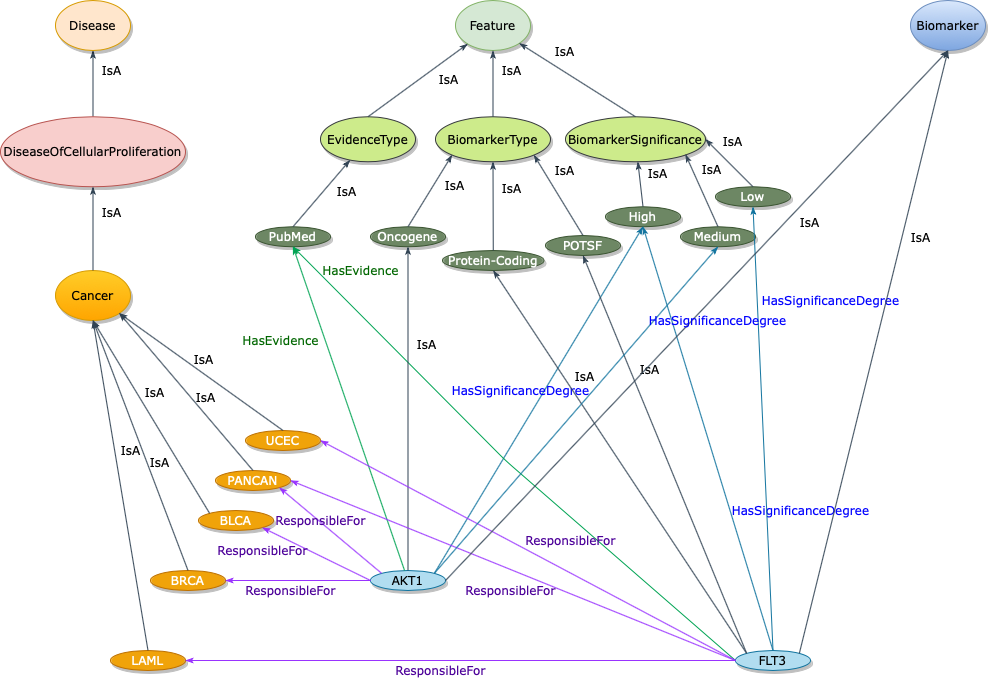
\includegraphics[width=0.8\linewidth,height=65mm]{images/GeneralRelations-Ontology.png}
	\caption{High-level view of the relations in the ontology}
	\label{fig:main_ontology_relations}
	\vspace{-2mm}
\end{figure*}

\hspace*{3.5mm} Classes from the DO are also treated as instances. Moreover, we included  the relation between a specific gene and one or more diseases. There are 3 main classes, which allow us to express the relation between entities. The general structure of the ontology is shown in \cref{fig:main_ontology}, while the hierarchical relations between the different classes and subclasses in the ontology are depicted as follows: \\

\vspace{-4mm}
{\scriptsize \noindent biomarker$\sqsubseteq$owl:Thing \\
BRCA1$\sqsubseteq$biomarker\\
Disease$\sqsubseteq$owl:Thing\\
BRCA$\sqsubseteq$Cancer$\sqsubseteq$DiseaseOfCellularProliferation$\sqsubseteq$Disease.}\\
\vspace{-4mm}

%\subsubsection{Cancer specific biomarkers}
\subsection{KG enrichment with cancer specific biomarkers} %Enriching disease specific knowledge}
Based on the inclusion and exclusion criteria in \cref{table:inclusion_exclusion_article}, cancer-related scientific articles are collected to extract information about cancer specific biomarkers from. For example, some genes exhibits both oncogenic and tumor-suppressor functionality~\cite{POSTF}. The KG can be enriched by extracting the name and properties of these genes. To extract such useful knowledge, a BERT-based information extraction method is employed. BioBERT and SciBERT variants of BERT are finetuned with the selected articles crawled from the PubMed, MeSH, CancerIndex, IEEE Digital Library, and Google Scholar. Our hypothesis is that, in learning to recover masked tokens, the model forms a representational topology of cancer-related unstructured sources will enable the ontology-guided knowledge extraction to outperform CRF and Bi-LSTM-based approaches for NER, entity-relationship extraction, and multi-type normalization tasks. 
%For the IE from \textbf{stream tables}, we will apply CascadeTabNet~\cite{cascadetabnet2020}, which is an end-to-end neural network architecture capable of both object detection and recognition simultaneously.

\subsubsection{Article inclusion and exclusion criteria}
Systematic reviews of complex evidence cannot rely solely on protocol-driven search strategies. Therefore, the literature began with the use of search queries with search terms and a Boolean operator such as ("cancer"[All Fields]) AND ("biomarkers "[All Fields]) and combining it with the snowball sampling searches. PubMed, MeSH, CancerIndex, IEEE Digital Library, and Google Scholar are used as the sources\footnote{Searching in Web of Sciences and Science Direct gave a few articles only.}, but by specifying more recent years~(i.e., 2010-2020). \Cref{table:inclusion_exclusion_article} shows the statistics of the systematic searching as of 12 February 2021. While using the protocol-based and snowball sampling-based searching, only one reason was recorded for each record, albeit multiple reasons were applicable. We excluded any manuscripts retrieved that were marked as drafts not to be cited. 

\begin{table*}[h!]
    \centering
    \caption{Cancer related article searching queries and related statistics}
    \label{table:inclusion_exclusion_article}
    \vspace{-2mm}
    \scriptsize{
    \begin{tabular}{p{0.75cm}|p{11cm}|p{0.6cm}|p{2.1cm}} 
        \hline
        \textbf{Query} & \textbf{Query string} & \textbf{\#hits} & \textbf{\#articles used} \\ 
        \hline
        Q1  & (``cancer''[All Fields] AND ``biomarkers''[All Fields]) OR (``oncology''[All Fields] AND ``biomarkers''[All Fields]) OR (``cancer genomics''[All Fields] AND ``biomarkers''[All Fields]) & 4,421 & 3,200 \\ 
        \hline
        Q2  & (``oncology''[All Fields] AND ``biomarkers''[All Fields]) OR (``cancer genomics''[All Fields] AND ``biomarkers”[All Fields]) OR(``cancer''[All Fields] AND ``oncogenes''[All Fields]) & 4,421 & 3,200 \\ 
        \hline
        Q3  & (``oncology''[All Fields] AND ``oncogenes''[All Fields]) OR (``cancer''[All Fields] AND ``biomarkers''[All Fields]) OR (``cancer genomics''[All Fields] AND ``biomarkers''[All Fields]) & 4,421 & 3,200 \\
        \hline
        Q4  & (``oncology''[All Fields] AND ``biomarkers''[All Fields]) OR (``cancer''[All Fields] AND ``cancer genomics''[All Fields]) OR (``cancer''[All Fields] AND ``biomarkers''[All Fields]) & 4,421 & 3,200 \\ 
        \hline
    \end{tabular}}
    \vspace{-4mm}
\end{table*}

\hspace*{3.5mm} As a continuation and following the search process using the queries in \cref{table:inclusion_exclusion_article}, all the records were merged, duplicates were removed, and a unique ID was assigned to each record. As we reused the word ``cancer'' in every search query, some overlapping results were returned as well. %Table 6 includes full texts from original search, snowball search (i.e. pursuing references of references) and reference list searches. 
Overall, based on the inclusion and exclusion criteria of the literature used for the systematic review, and based on the outcome, we used only selected research papers that were more relevant, recent and highly cited. Since the systematic review was conducted a few months back, depending on the contents, addition or deletion  to/from  the above databases might happen.Consequently, the same queries may return a different results.

\subsubsection{Article preprocessing}
The pre-processing task involved, tokenisation, part-of-speech~(PoS) tagging, stemming, removal of stop words, dependency parsing, word sense disambiguation, linking words: 

\begin{enumerate}[noitemsep]
    \item \textbf{Tokenisation} - it involves parsing the text into atomic terms, words, and symbols. 
    \item \textbf{Stemming} - it is about reducing tokens into their stem, base or root form. 
    \item \textbf{Stop words removal} - it is about removing insignificant words. 
    \item \textbf{PoS tagging} - to identify terms representing verbs, nouns, adjectives, etc. 
    \item \textbf{Dependency parsing} - is about extracting a grammatical tree structure for a sentence where leaf nodes indicate individual words that together form phrases. 
    \item \textbf{Word sense disambiguation} - to identify the meaning in which a word is used. 
    \item \textbf{Linking words} -linking terms with a lexicon of senses based on a domain-specific ontology. 
\end{enumerate}

\hspace*{3.5mm} The linking of words is mostly involved entity linking, which is done in a later step. The resulting cleaned texts are then represented in  the CoNLL format\footnote{\url{http://universaldependencies.org/docs/format.html}}, where a corpus is represented with one word per line, each word containing 10 tab-separated columns with information about the word. 

\subsubsection{Bio-entity extraction}
The bio-entity extraction component involve two tasks: i) NER that recognizes the named entities in PubMed abstracts based on BioBERT~\cite{BioBERT} and SciBERT~\cite{SciBERT} models, ii) entity linking to link extracted named entities, and iii) relation extraction. Named entity recognition~(NER) is about recognizing domain-specific proper nouns in a biomedical corpus. For example, for the sentence \texttt{The main proteins regulating cell-cycle are BAD and PNCa, which have downstream effects}, proteins, cell-cycle, BAD, and PNCa are 4 proper nouns. \texttt{TP53 and FAS are top two POTSF genes in terms of the number of associated cancer types, which are associated with 34 and 15 cancer types}, is another example, where a NER model is able to identify that TP53, FAS, POTSF genes, and cancer are the named entities. Recent NER approaches extract such named entities based on learning frameworks that leverage lexical features such as POS tags, dependency parse trees, etc~\cite{hogan2020knowledge}. 
    
\hspace*{3.5mm} The entity linking is about associating mentions of the named entities in a text with the existing nodes of our target KG~\cite{hogan2020knowledge}. Assuming these entities already exist in the KG, entity linking module then links the given mentions to these nodes. The entity linking task also involves named entity disambiguation, e.g., given that there could be multiple ways to mention the same entity~(e.g., \texttt{p53} and \texttt{TP3} are synonymously used). In such a case, the information available under both mentions across different nodes are splitted, under the assumptions that various aliases and multilingual labels are already captured during the NER task. Further, depending upon the complexity in the NER task, multi-type normalization are performed to assign unique IDs to extracted bio entities. Finally, the relation extraction, which is task to extract relations between the extracted entities is performed. In our case, both binary and n-ary relation types are considered only, in a closed setting where in a fixed set of relation types.  

\begin{figure*}
	\centering
	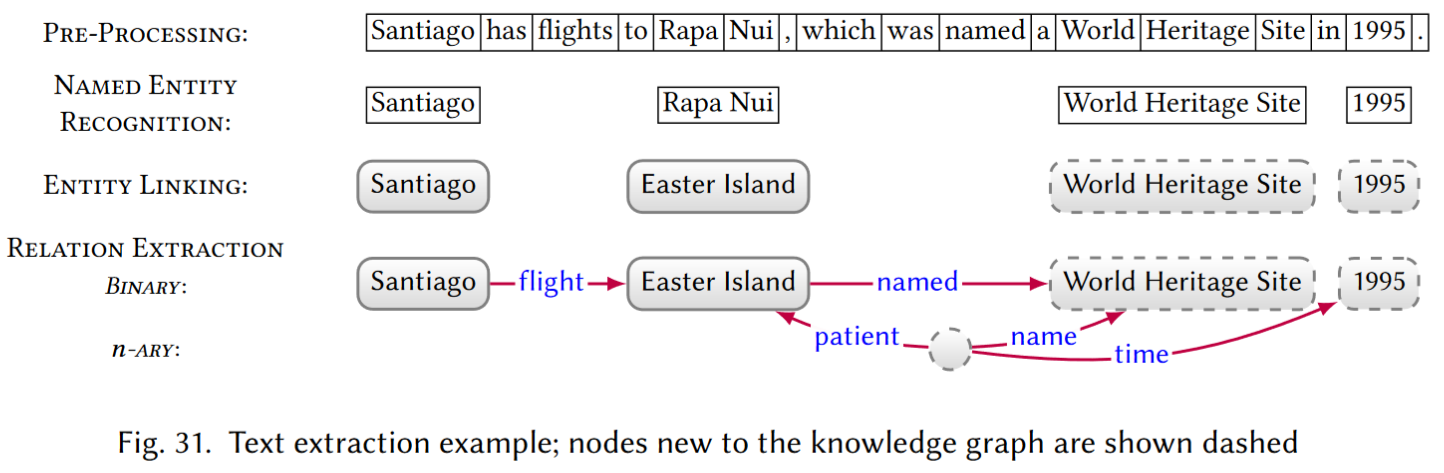
\includegraphics[scale=0.8]{images/ner.png}
	\caption{ Text extraction example; nodes new to the knowledge graph are shown dash}
	\label{fig:ner_pipeline}
	\vspace{-2mm}
\end{figure*}

\subsubsection{Fine-tuning NER models}
The transformers in all the BERT variants connect the encoders and decoders through self-attention for greater parallelization and reduced training time~\cite{hasan2020knowledge,kim2019neural}. BERT was originally pre-trained on English Wikipedia, news, and book corpus. Thus, it requires domain-specific finetuning for biomedical domain texts that contain a considerable number of domain-specific proper nouns and terms. Recently, BioBERT and SciBERT are recently finetuned for solving different biomedical tasks, as shown in \cref{fig:ner_bert_pipeline}. Both variants for BERT are found to be very effective at recognizing known biomedical entities~\cite{kim2019neural}. 

\begin{figure*}
	\centering
	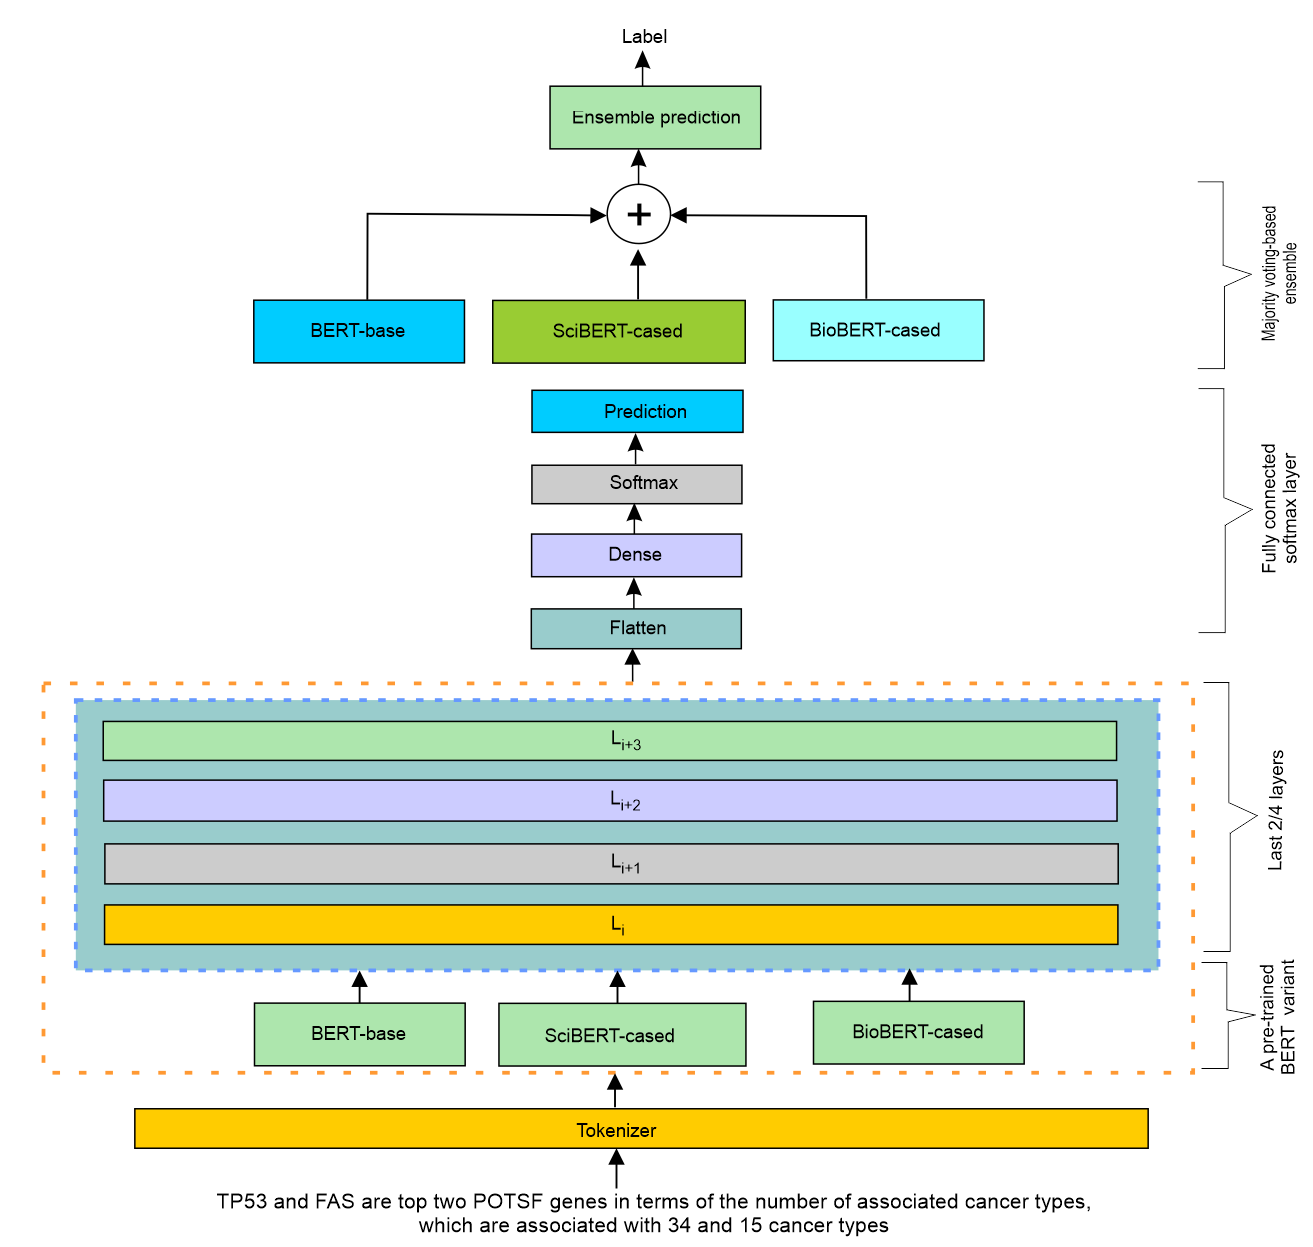
\includegraphics[scale=0.85]{images/ner_bert.png}
    \caption{A schematic representation of the NER task, where each of three different transformer variants are finetuned by adding a fully connected softmax layer on top, followed by voting-based ensemble prediction}
	\label{fig:ner_bert_pipeline}
	\vspace{-2mm}
\end{figure*}

\hspace*{3.5mm} BioBERT and SciBERT are initialized with case-sensitive version of BERT~(i.e., BERT cased). Then the SciBERT and BioBERT's weights are pre-trained on PubMed articles. Each pre-trained model are further fine-tuned for the NER task based on the selected articles that are collected based on the criteria defined in \cref{table:inclusion_exclusion_article}. While fine-tuning BioBERT and SciBERT,  WordPiece\footnote{WordPiece embedding is a method of dividing and expressing a word into masked tokens.} tokenization is used to mitigate the out-of-vocabulary issue. The NER models available in SciBERT and BioBERT can predict the following seven tags~\cite{kim2019neural}: 

\begin{enumerate}[noitemsep]
    \item \textbf{IOB2 tags} - Inside, Outside, and Begin. 
    \item \textbf{X} - sub-token of WordPiece.  
    \item \textbf{[CLS]} - the leading token of a sequence for classification. 
    \item \textbf{[SEP]} - a sentence delimiter.  
    \item \textbf{PAD} - a padding of each word in a sentence. 
\end{enumerate}

The BertTokenizer was applied to words in a sentence on a dataset~(i.e., in CoNLL format) with labels. The WordPiece algorithm\footnote{\url{https://huggingface.co/transformers/tokenizer_summary.html}} was then applied to the sub-words of each word. BioBERT was able to extract diverse types of bio-entities, where an entity or two entities with frequently-occurring token interaction would be marked with more than one entity type span. Based on the calculated probability distribution, we were able to choose the correct entity type when entities were tagged with more than two types according to the probability-based decision rules~\cite{kim2019neural}. The NER models were fine-tuned as follows~\cite{kim2019neural}:

\begin{align}
    p\left(T_{i}\right)=\operatorname{softmax}\left(T_{i} W^{T}+b\right)_{k},
\end{align}

\hspace*{3.5mm} where $k$ represents the indexes of seven tags $\{\mathrm{B}, \mathrm{I}, \mathrm{O}, \mathrm{X},[\mathrm{CLS}],[\mathrm{SEP}], \mathrm{PAD}\}, p$ is the probability distribution of assigning each $k$ to token $i$, and $T_{i} \in R^{H}$ is the final hidden representation. The final hidden representation is calculated by BioBERT and SciBERT for each token $i$, $H$ is the hidden size of $T_{i}, W \in R^{K \times H}$ is a weight matrix between $k$ and $T_{i}, K$ represents the number of tags and is equal to $5$, and $b$ is a $\mathrm{K}$ -dimensional bias vector on each $k$. The classification loss $L$ is calculated as follows~\cite{kim2019neural}:

\begin{align}
    L(\Theta)=-\frac{1}{N} \sum_{i=1}^{N} \log \left(p\left(y_{i} \mid T_{i}; \Theta\right)\right. ,
    \label{eq:bert_class_loss}
\end{align}

\hspace*{3.5mm} where $\Theta$ represents the trainable parameters, and $N$ is the sequence length. During the fine-tuning for 20 epochs, the training set is shuffled for every epoch, gradient clipping is applied, the initial learning rate is set to $2 e^{-5}$, the Adam optimizer is used to optimize the loss~(i.e., \cref{eq:bert_class_loss}) with the scheduled learning rate.  Then the multi-head attention layer is followed by a fully-connected softmax layer. \Cref{table:bert_params} shows the hyperparameter combination. 
%For the pre-training of \textit{BERT-cased} model, the maximum input length is set to $256$. 

\begin{table*}
    \centering
    \caption{Hyperparameter combination for BERT variants}
    \label{table:bert_params}
    \begin{tabular}{l|l|l|l|l}
        \hline
        \textbf{Hyper parameter}  & \textbf{BioBERT cased} &
        \textbf{SciBERT cased} & \textbf{BERT cased}\\
        \hline
        Learning rate & 3e-5 & 5e-5 & 2e-5 \\
        Epochs & 6 & 6 & 5 \\
        Max sequence length & 128 & 128 & 128 \\
        Dropout & 0.3 & 0.3 & 0.4 \\
        Batch size & 16 & 16 & 16 \\
        \hline
    \end{tabular}
\end{table*}

\subsubsection{Integrating extracted triples into KG}
Possible sub-classes of `BiomarkerSignificance' is defined as HIGH, MEDIUM, and LOW based on the annotations provided in the TumorPortal\footnote{\url{http://www.tumorportal.org/tumor_types?ttype=PanCan}}. Further, each entity belonging to the class biomarker is annotated with the properties available in the OGG ontology, as shown in \cref{fig:ogg_ontology}. Besides, number of scientific articles is included as an evidence associated with certain genes, which is shown in \cref{fig:biomarker_subclass}. The `Disease' class consists of a subclass named `DiseaseOfCellularProliferation' under which there is another sub-class called `Cancer'. Under the class Cancer we included those 33 cancer types of interests, and which are labeled with their well-known abbreviations, e.g., BRCA for breast cancer. \Cref{fig:diseases_class} shows the structure of the class disease and its subclasses. For the entities in the class disease, object properties from the DOID ontology are also inherited and included as annotations. 

\begin{figure*}[h]
	\centering
		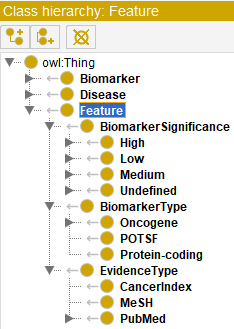
\includegraphics[width=0.3\linewidth,height=60mm]{images/feature_class.png}
        \label{fig:biomarker_subclass}
	\caption{Annotations and relations between entities in the biomarker class and subclass}
	\vspace{-2mm}
\end{figure*}

\hspace*{3.5mm} The class `Feature' is included expressing the relation between a disease and the responsible genes, as shown in \cref{fig:biomarker_subclass}. We indicate the significance degree of a particular gene w.r.t a disease. Besides, the biomarker type and the evidence type information are also included, where PubMed, MeSH, and CancerIndex are considered as the source of the evidence. These features~(in terms of annotations and object properties) are used to indicate the relation between entities from different classes, as shown in \cref{fig:biomarker_subclass}, which in turn annotations allow the rules generation. Furthermore, since depending on the types gene biomarkers can be categorized as `Oncogene', `Protein-coding', and `POTSF', we considered these as the subclasses of `BiomarkerType'. 

\begin{figure*}
	\centering
	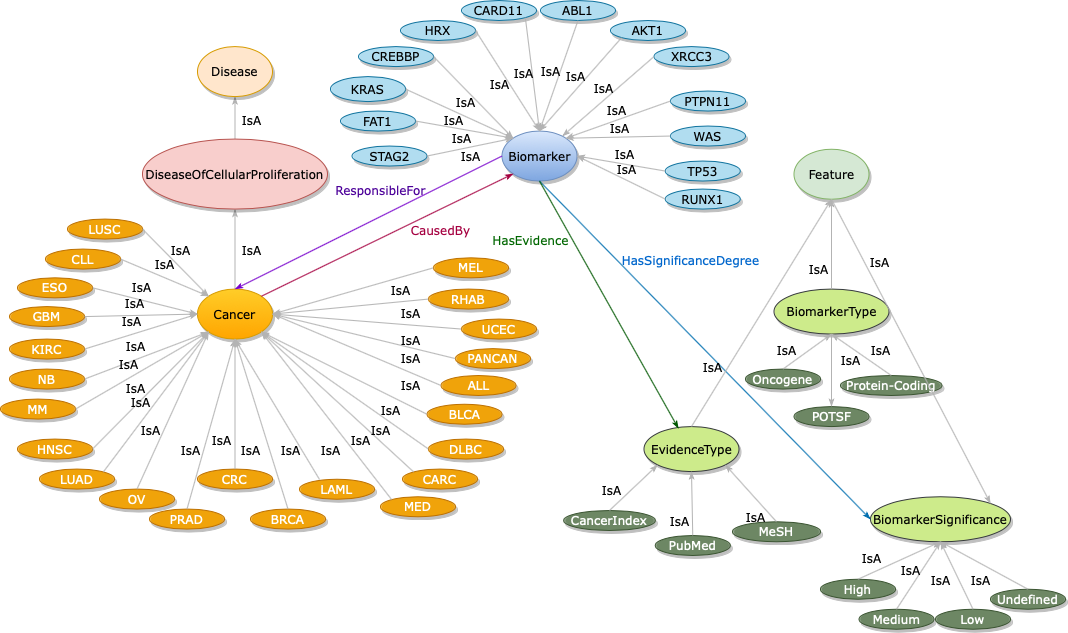
\includegraphics[width=0.8\linewidth,height=60mm]{images/diagram_general_view.png}
	\caption{High-level view of the ontology} 
	\label{fig:main_ontology}
\end{figure*}

\hspace*{3.5mm} In the relation extraction step, links between extracted lexical terms from the source text and the concepts from the ontology is defined. Then, using a BioBERT and SciBERT-based NER module, the context of the terms will be analyzed to determine the appropriate disambiguation, before assigning the term to the correct concept. Finally, attribute-value pairs are identified, which involves the identification of a subject, mapping it to a semantic class, and using the predicate and object as the attribute name and value, respectively. \Cref{fig:main_ontology_pro_view} shows the hierarchical view of the biomarker class, where we included all the biomarkers, particularly, genes related to all the cancer types we consider in this ontology. 

\begin{figure*}[h]
	\centering
		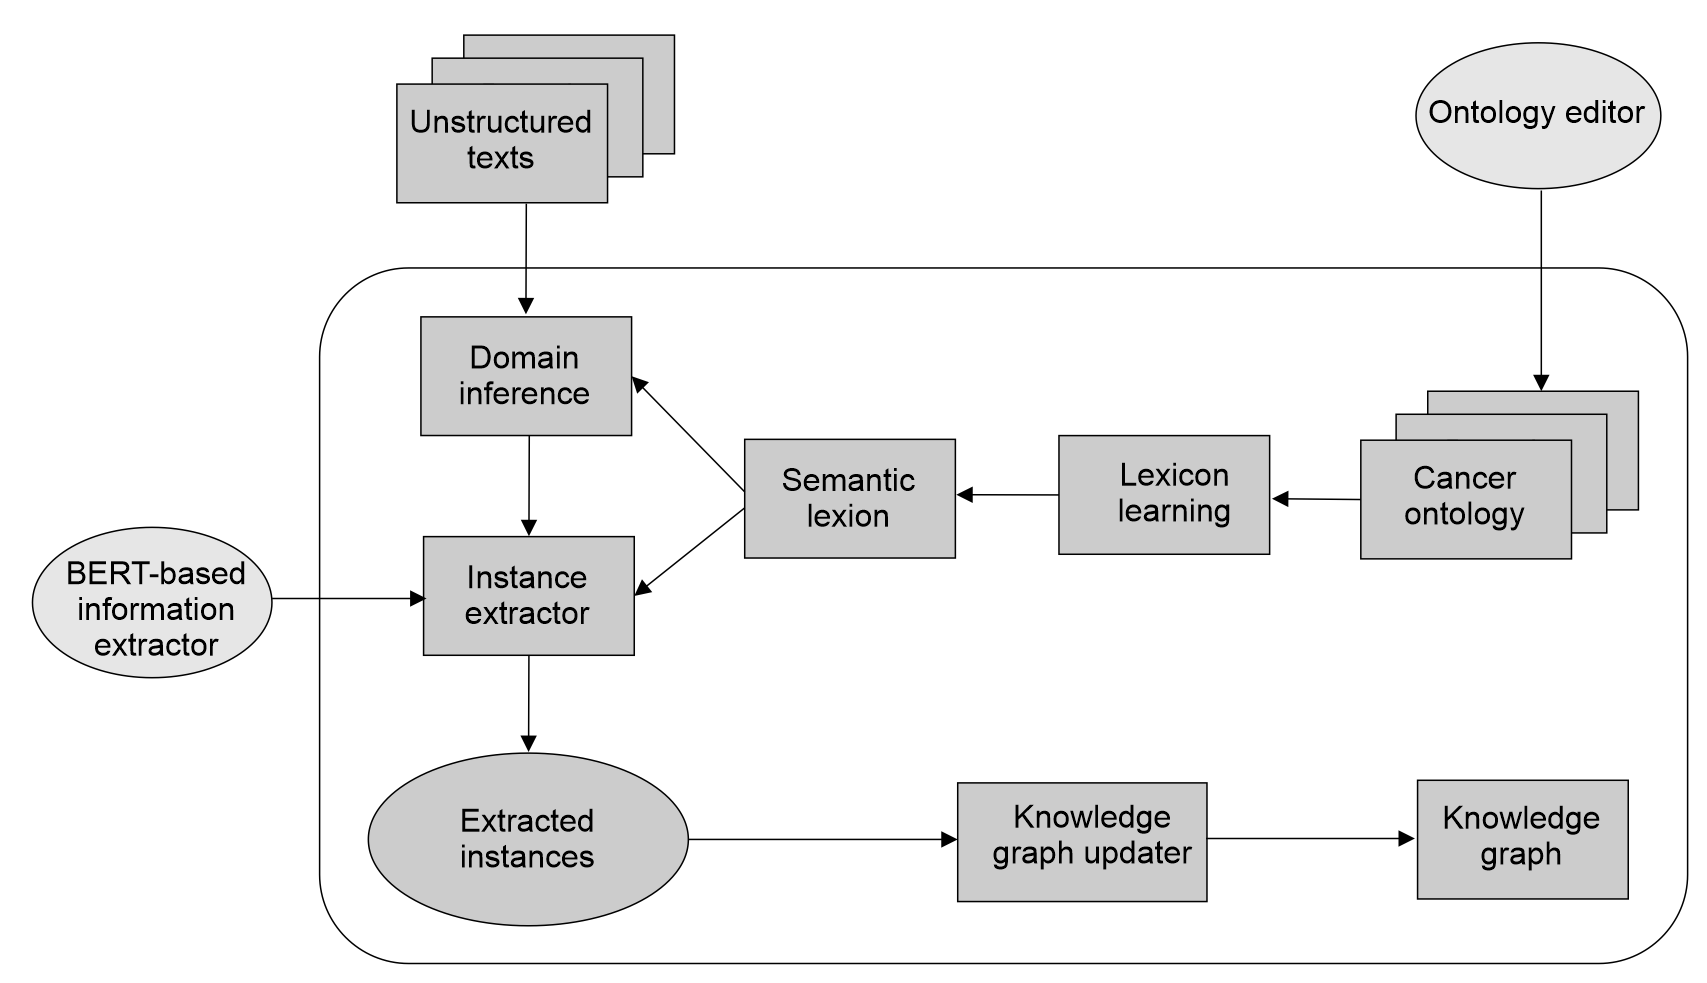
\includegraphics[scale=0.65]{images/KG_enrichment.png}
        \label{fig:kg_enrichment}
	\caption{Knowledge graph enrichment with cancer specific biomarkers}
	\vspace{-2mm}
\end{figure*}

\hspace*{3.5mm} To integrate the new information into the KG, a semantic lexicon is incorporated. The lexicon extractor is a BioBERT and SciBERT-based instance extractor, which: i) uses the rules from the cancer ontology to enrich the semantic lexicon with new lexicon symbols and ii) extracts the instance information and create RDF triples, followed by enrichment of the KG. In our approach, each instance is extracted as an RDF triple in the form of $(u,e,v)=(\mathit{subject},\mathit{predicate},\mathit{object})$, where each triple forms a connected component of a sentence for the KG. 

\hspace*{3.5mm} As many as 83 POTSF genes 
%reported by Shen et al.~\cite{POSTF} through database search and literature annotation are used to enrich the list. 
have been identified: 
BRCA1, CAMTA1, CBFA2T3, CDX2, CREB3L1, CREBBP, DDB2, DNMT1, DNMT3A, ETV6, EZH2, FOXA1, FOXL2, FOXO1, FOXO3, FOXO4, FOXP1, FUS, IRF4, KLF4, KLF5, NCOA4, NOTCH1, NOTCH2, NOTCH3, NPM1, NR4A3, PAX5, PML, PPARG, RB1, RUNX1, SMAD4, STAT3, TCF3, TCF7L2, TP53, TP63, TRIM24, WT, ZBTB16, BCR, CHEK2, EPHA1, EPHA3, EPHB4, FLT3, MAP2K4, MAP3K4, MST1R, NTRK3, PRKAR1A, PRKCB, SYK, ARHGEF12, BCL10, BRCA2, CBL, CDC73, CDH11, CDKN1B, DCC, DDX3×, DICER1, FAS, FAT1, GPC3, IDH1, IKZF2, LIFR, NF2, NUP98, PHF6, PTPN1, PTPN11, RHOA, RHOB, SH2B3, SLC9A3R1, SOCS1, SPOP, SUZ12, WHSC1L1. 

\iffalse
\begin{figure*}[h]
	\centering
	\begin{subfigure}{.48\linewidth}
		\centering
		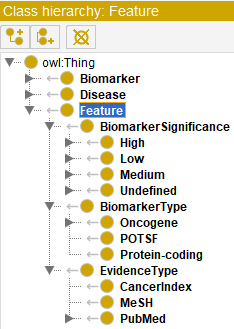
\includegraphics[width=0.6\linewidth,height=60mm]{images/feature_class.png}
		\caption{Biomarker class}
        \label{fig:feature_class}
	\end{subfigure}
	\begin{subfigure}{0.48\linewidth}
		\centering
		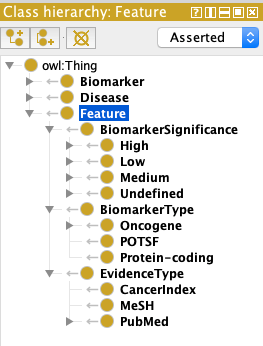
\includegraphics[width=0.6\linewidth,height=60mm]{images/feature1.png}
		\caption{Biomarker subclass}
        \label{fig:biomarker_subclass}
	\end{subfigure}
	\caption{Annotations and relations between entities in the biomarker class and subclass}
	\label{fig:biomarker_class_subclass}
	\vspace{-2mm}
\end{figure*}
\fi 

%\subsubsection{Enriching gene specific evidence}
\subsubsection{KG quality assessment}
Modelling ontologies is one of the key topics in knowledge engineering because of the difficulties it involves~\cite{poveda2014oops}. Regardless the source from which the data is collected, KG is created, and data extracted for the initial KG will usually be incomplete, and will contain duplicate, anomalies or errors, contradictory or even incorrect statements – especially when taken from multiple sources~\cite{hogan2020knowledge}. Therefore, once the KG is constructed and enrichment of a KG from external sources, a crucial step is to assess the quality of the resulting KG for fitness of purpose. Ensuring the robustness of a constructed KG is of utmost significance to ensure the quality of the inferred knowledge. The proliferation of massive KGs poses a question on the quality of the embedded knowledge~(i.e., entities and relations), and whether these facts precisely depict the intended real-world concepts and their relationships.

\hspace*{3.5mm} In graph theory, one of the most established approaches to finding the most important nodes is the centrality indicators. Centrality measures such as closeness-, betweenness-, and eigenvector centrality are used to determine the most influential node in a social network. However, these measures do not take into consideration the node attributes~\cite{zhang2018link}. Zhang et al.~\cite{zhang2018link} showed that a two or three neighborhood subgraph around a targeted link is sufficient to predict its attribute values. For example, in our CE context, this can be related to missing thermodynamic stream properties of stream in a flowsheet.
Classification and ranking metrics such as Hits@N and mean reciprocal rank, accuracy, precision, recall, and F-score~\cite{Morris2019} that have been currently incorporated to evaluate the KG construction and completion in terms of the factuality of the embedded entities and their relations~\cite{karim2019drug}.

\hspace*{3.5mm} However, since such comprehensive quality assessment are subject to other downstream tasks based on KG embeddings, this thesis consider them out of the scope. Instead a lightweight measure is taken to evaluate the integrated ontology in order to detect possible inconsistencies using \texttt{OntOlogy Pitfall Scanner!}~(OOPS)~\cite{poveda2014oops} and avoid them. OOPS helped us\footnote{\url{http://oops.linkeddata.es/}}: 

\begin{enumerate}[noitemsep]
    \item The domain or range of a relationship is defined as the intersection of two or more classes. This warning could avoid reasoning problems in case those classes could not share instances. 
    \item No naming convention is used in the identifiers of the ontology elements. In this case the maintainability, the accessibility and the clarity of the ontology could be improve.
    \item A cycle between two classes in the hierarchy is included in the ontology. Detecting this situation could avoid modelling and reasoning problems.
\end{enumerate}

\subsection{Ontological reasoning: query processing to instance classification}
As already stated, our semantic layer, consists of four components: query processing module, knowledge matching module, instance classifier, and the ontology reasoner. The ontology represented as a RDF KG consists of 31,034 triples including data, ontologies, and formal representation annotations. The semantic layer provides an interface between the KG and the rule generator. %We provide the details of each component in this sub-section.

\subsubsection{Query processing}
Having extracted a set of concepts from the decision rules, we relate them to the KG in SPARQL or DLx query format. For the former, concepts are stored as RDF triples and queried via SPARQL endpoint. For the latter, we query via Prot{\'e}g{\'e}\footnote{An open-source tools to construct domain models and knowledge-based applications with ontologies, Link: \url{https://protegewiki.stanford.edu/wiki/Main_Page}} DLx query view. 
%\subsubsection{Query formulation}
With all concepts mapped to KB entities, the next step is forming queries in SPARQL or DLx formats, depending on the question template. 
A human agent or end users like clinicians/doctors may require to formulate the query in a convenient way. However, for the simplicity, we focus on the DLx queries, albeit SPARQL is definitely our outlook for the better expressivity. The next step is then to generate answers according to the results of the queries, where the reasoner searchers concepts in the KG that are already classified w.r.t entity types, which we use to give ``logical reasons" as to how the answer is generated. Especially, for questions requiring external knowledge, the predicates and entities on the path give a better understanding of how the relationships are established between the concepts from the rule and and KB concepts. 

\subsubsection{Instance classification and reasoning}
In order to perform reasoning in forward chaining in presence of rules, the reasoner applies all the rules in the rule-base on the set of facts in the factual part then query the KG in a classical manner.
In many cases, a set of facts $\mathcal{F}$ may contain contradictory knowledge, giving inconsistencies. We say that a set of facts is inconsistent if an only if  $\mathrm{Cl}_{\mathcal{R}}(\mathcal{F})$ triggers a negative constraint~\cite{garoufallou2016metadata}. For the simplicity, we assume that our rule-base does not contain contradictory rules. There are two distinct types of entities: biological entities and classes from biomedical ontologies that provide background knowledge about entities. 

\hspace*{3.5mm} Ontology-based annotations are expressed by asserting a relation between the instance, e.g., a gene and cancer types and an instance of the ontology class. For example, we express that gene $AKT1$ has the GO association \texttt{GO:0000060} by two axioms \texttt{hasGOAssociation(AKT1,$f_1$)} and \texttt{instanceOf($f_1$, GO:0000060)}: $AKT1$ and $f_1$ are instances, \texttt{GO:0000060} is a class \url{http://purl.obolibrary.org/obo/GO\_0000060} in GO, \texttt{hasGOAssociation} is an object property, and \texttt{instanceOf} is the \texttt{rdf:type} property in OWL standard. Each instance $f_i$ in the KG is assigned a unique IRI. The OWL2 EL standard is followed for representing KGs and utilize different reasoners such as Pellet, HermiT, and ELK for automated reasoning over them. OWL2 EL that supports basic inferences over ontological class hierarchies and object properties, can infer the classification of instances, via  the class descriptions, class axioms, and object property axioms~\cite{alshahrani2017neuro}: 

\begin{itemize}[noitemsep]
\vspace{-2mm}
    \item \textbf{Class description} - class intersection $(A \sqcap B)$, existential quantification $(\exists r . A),$ limited enumeration using a single instance $\left(\left\{x_{i}\right\}\right)$. 
    \item \textbf{Class axioms} - $E_{1}$:$E_{2}$ indicates entity $E_{1}$ is an instance of class $E_{2}$, subclass $(A \sqsubseteq B)$\footnote{Means concept $A$ is subsumed by concept $B$}, equivalent class $(A \equiv B)$, disjointness $(A \sqcap B \sqsubseteq \perp)$. 
    \item \textbf{Object property axioms} - sub-property $(r \sqsubseteq s)$, property chains $(r \circ s \sqsubseteq q)$, equivalent property $(r \equiv s)$, transitive properties $(r \circ r \sqsubseteq r)$, reflexive properties. 
    \vspace{-2mm}
\end{itemize}

\hspace*{3.5mm} We use the Pellet reasoner to deductively close the KG, i.e., we deductively close our KG w.r.t. the OWL2 EL profile. The $\mathcal{KG}$ would be deductively closed $iff$ for all $\phi$ s.t. $\mathcal{KG} \models \phi, \phi \in \mathcal{KG}$. Although the deductive closure of a knowledge is countably infinite, we assume it is finite for our case. Subsequently, we add only inferences that can be represented explicitly as edges between named individuals and classes~(i.e., entities that are explicitly named) in the $\mathcal{KG}$ s.t. for all instances $x_{i}, x_{j} \in \mathcal{KG}$ and object properties $r \in \mathcal{KG}$, if $\mathcal{KG} \models r\left(x_{i}, x_{j}\right)$, then $r\left(x_{i}, x_{j}\right) \in \mathcal{KG} ^{\models}$. Furthermore, for all named classes $C \in \mathcal{KG}$ and instances $x \in \mathcal{KG}$, if $\mathcal{KG}=\mathrm{C}(x)$, then $C(x) \in \mathcal{KG} ^{\pm}$. Finally, relations between classes are inferred by adding subclass axioms to the inferred graph, s.t. for any class $C, D \in \mathcal{KG}$, if $\mathcal{KG} \models C \sqsubseteq D$, then $C \sqsubseteq D \in \mathcal{KG}^{\pm}$. 

\section{Experiments}\label{chapter_8:results}
In this section, we discuss the evaluation results, both quantitatively and qualitatively. Besides, a comparative analysis with state-of-the-art approaches is provided. More specifically, several experiments were carried out to improve the adversarial robustness of the models, with the following objectives:

\begin{enumerate}[noitemsep]
    \item Can we train a surrogate model to approximate the behaviour of a complex DNN model? 
    \item How effective a surrogate model at approximating the oracle model?  
    \item How effective decision rules are to explain global and local behaviours of a model?   
    \item Can we explain misclassified instances using decision rules? 
\end{enumerate}

\hspace*{3.5mm} Results of each observation are analysed, both quantitative and qualitatively, in the following section.

\subsection{Experiment setup}
We used Prot{\'e}g{\'e} 5.5.0 is used for the reasoning, DLx querying, and DL rule generations with Pellet, RLK, and HermiT reasoners. 
%The detail information including versions are shown in \cref{fig:plugins_info}. 
However, ELK does not support object all values from axioms, while HermiT gave some inconsistent~(giving different number of rules). Therefore, we report the rules generated with Pellet only. The inferred rules based on the reasoning are expressed using DLx format. To evaluate the effectiveness of domain-specific potentials of transformer-based approach for information extraction, a comparative analysis with the well-established CRF and Bi-LSTM architectures. 

\subsection{Query benchmarks}
Below we provide a few questions in human language~(NLQ) and in DLx query~(DLQ) format. The answers based on different reasoners can be found in appendix. However, as shown in in \cref{fig:sample_q_a}, the answer of NLQ ``List of all biomarkers which are classified POTSF and responsible for breast cancer answered" against the DLQ ``Biomarker and responsible\_for some BRCA and is\_a only POTSF" by the Prot{\'e}g{\'e} is understandable but not clear how the reasoner derives such answer. Therefore, in the next subsection, we derive corresponding rule for individual biomarker. 

\iffalse
\begin{sidewaystable*}
    \caption{Example of gene expression samples based on oncogenes}
    \label{table:nlq_dlq}
    \vspace{-6mm}
    \begin{center}
        \scriptsize
        \begin{tabular}{l|l}
            \hline
            \rowcolor{Gray}
            \textbf{NLQ} & \textbf{DLQ} \\\hline  
                What is BLCA? & BLCA \\\hline
                What is Cancer? & Cancer \\\hline
                List of all biomarkers? & Biomarker \\\hline
                Which biomarkers have PubMed evidence associated? & has\_evidence \textcolor{blue}{some} PubMed \\\hline
                List of Oncogene, POTSF, and Protein-Coding biomarkers? & Biomarker \textcolor{green}{and} is\_a only Oncogene \textcolor{green}{and} is\_a only POTSF \textcolor{green}{and} is\_a only Protein-coding \\\hline
                List of Oncogene biomarkers responsible for Medulloblastoma with evidence? & Biomarker \textcolor{green}{and} responsible\_for \textcolor{blue}{some} MED \textcolor{green}{and} is\_a only Oncogene \textcolor{green}{and} (has\_evidence \textcolor{blue}{some} PubMed \textcolor{red}{or} has\_evidence \textcolor{blue}{some} CancerIndex \textcolor{red}{or} has\_evidence \textcolor{blue}{some} MeSH) \\\hline
                List of Oncogene, POTSF, and Protein-coding biomarkers responsible for breast cancer? & Biomarker \textcolor{green}{and} responsible\_for \textcolor{blue}{some} BRCA \textcolor{green}{and} is\_a only Oncogene \textcolor{green}{and} (is\_a only POTSF \textcolor{red}{or} is\_a only Protein-coding) \\\hline                
                List of Oncogene biomarkers responsible for breast cancer? & Biomarker \textcolor{green}{and} responsible\_for \textcolor{blue}{some} BRCA \textcolor{green}{and} is\_a only Oncogene \\\hline
                List of POTSF biomarkers responsible for breast cancer? & Biomarker \textcolor{green}{and} responsible\_for \textcolor{blue}{some} BRCA \textcolor{green}{and} is\_a only POTSF \\\hline
                List of biomarkers that have at least 5 scientific articles as PubMed evidence? & Biomarker \textcolor{green}{and} has\_evidence \textcolor{blue}{some} PubMed \textcolor{green}{and} has\_citations min 5 \\\hline
                List of biomarkers that have maximum 100 scientific articles associated? & Biomarker \textcolor{green}{and} has\_citations max 100 \\\hline
                Which cancer types caused by biomarker ERBB2? & Cancer \textcolor{green}{and} caused\_by \textcolor{blue}{some} ERBB2 \\\hline
                Which cancer types caused by biomarker TP53? & Cancer \textcolor{green}{and} caused\_by \textcolor{blue}{some} TP53 \\\hline
                Which biomarkers have significance degree High? & Biomarker \textcolor{green}{and} has\_significance\_degree \textcolor{blue}{some} High \\\hline
                Which biomarkers have significance degree High and responsible for BLCA cancer? & Biomarker \textcolor{green}{and} responsible\_for \textcolor{blue}{some} BLCA \textcolor{green}{and} has\_significance\_degree \textcolor{blue}{some} High \\\hline
        \end{tabular}
        \vspace{-4mm}
    \end{center}
\end{sidewaystable*}
\fi 

\begin{sidewaystable*}
    \caption{Example of gene expression samples based on oncogenes}
    \label{table:nlq_dlq}
    \vspace{-4mm}
    \begin{center}
        \scriptsize
        \begin{tabular}{l|l}
            \hline
            \rowcolor{Gray}
            \textbf{NLQ} & \textbf{DLQ} \\\hline  
                What is BLCA? & BLCA \\\hline
                What is Cancer? & Cancer \\\hline
                List of all biomarkers? & Biomarker \\\hline
                Which biomarkers have PubMed evidence associated? & has\_evidence \textcolor{blue}{some} PubMed \\\hline
                List of Oncogene, POTSF, and Protein-Coding biomarkers? & Biomarker \textcolor{green}{and} is\_a only Oncogene \textcolor{green}{and} is\_a only POTSF \textcolor{green}{and} is\_a only Protein-coding \\\hline
                List of Oncogenes responsible for Medulloblastoma with evidence? & Biomarker \textcolor{green}{and} responsible\_for \textcolor{blue}{some} MED \textcolor{green}{and} is\_a only Oncogene \textcolor{green}{and} (has\_evidence \textcolor{blue}{some} PubMed \textcolor{red}{or} CancerIndex \textcolor{red}{or}  MeSH) \\\hline
                List of Oncogene, POTSF, and Protein-coding genes for breast cancer? & Biomarker \textcolor{green}{and} responsible\_for \textcolor{blue}{some} BRCA \textcolor{green}{and} is\_a only Oncogene \textcolor{green}{and} (is\_a only POTSF \textcolor{red}{or} is\_a only Protein-coding) \\\hline              
                List of Oncogene biomarkers responsible for breast cancer? & Biomarker \textcolor{green}{and} responsible\_for \textcolor{blue}{some} BRCA \textcolor{green}{and} is\_a only Oncogene \\\hline
                List of POTSF biomarkers responsible for breast cancer? & Biomarker \textcolor{green}{and} responsible\_for \textcolor{blue}{some} BRCA \textcolor{green}{and} is\_a only POTSF \\\hline
                List of biomarkers with at least 5 articles as PubMed evidence? & Biomarker \textcolor{green}{and} has\_evidence \textcolor{blue}{some} PubMed \textcolor{green}{and} has\_citations min 5 \\\hline
                List of biomarkers with maximum 100 articles associated? & Biomarker \textcolor{green}{and} has\_citations max 100 \\\hline
                Which cancer types caused by biomarker ERBB2? & Cancer \textcolor{green}{and} caused\_by \textcolor{blue}{some} ERBB2 \\\hline
                Which cancer types caused by biomarker TP53? & Cancer \textcolor{green}{and} caused\_by \textcolor{blue}{some} TP53 \\\hline
                Which biomarkers have significance degree High? & Biomarker \textcolor{green}{and} has\_significance\_degree \textcolor{blue}{some} High \\\hline
                Which biomarkers have significance degree High for BLCA cancer? & Biomarker \textcolor{green}{and} responsible\_for \textcolor{blue}{some} BLCA \textcolor{green}{and} has\_significance\_degree \textcolor{blue}{some} High \\\hline
        \end{tabular}
        \vspace{-2mm}
    \end{center}
\end{sidewaystable*}

\begin{figure*}
	\centering
	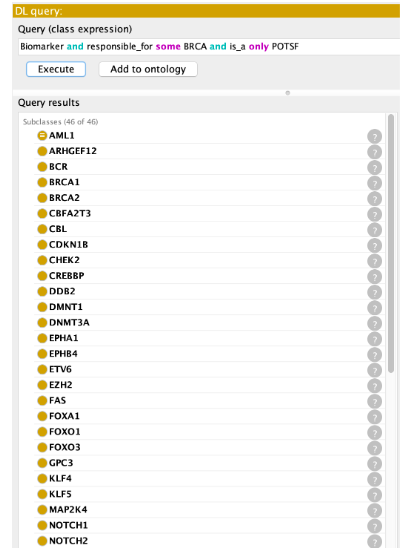
\includegraphics[width=0.45\linewidth,height=70mm]{images/sample_q_a.png}
	\caption{List of biomarkers classified as POTSF and responsible for breast cancer answered}
	\label{fig:sample_q_a}
	\vspace{-2mm}
\end{figure*}

\iffalse
\begin{figure}[th]
\vspace{-2mm}
\centering
\scriptsize
\begin{Verbatim}[frame=lines,numbers=left,numbersep=1pt]
SELECT ?otherEntity (count(?tweet) as ?count) WHERE {
  ?tweet schema:mentions ?entity ; dc:created ?date 
                FILTER(year(?date) = 2020 AND month(?date) = 4) .
  ?entity a nee:Entity ; nee:hasMatchedURI dbr:Donald_Trump .
  ?tweet schema:mentions ?entity2 . 
  ?entity2 a nee:Entity ; nee:hasMatchedURI ?otherEntity 
                FILTER (?otherEntity != dbr:Donald_Trump)
} GROUP BY ?otherEntity order by desc(?count) LIMIT 5
\end{Verbatim}
\vspace{-3mm}
\caption{Top entities co-occurring with the entity \textit{Donald Trump} during April 2020.}
\label{fig:sparqlEx1}
\vspace{-3mm}
\end{figure}
\fi 

\subsection{Interpretation of generated rules}
We interpret the inferred rules. We apply DLx Class Axiom Renderer Plugin\footnote{\url{https://github.com/MindfulMichaelJames/ProtegeDLAxiomPlugin}} to represent the rules.   
\subsubsection{Notations and assumptions}
Due to brevity, we cover some notations and assumptions that will be used for the interpretations:

\noindent i) if <Biomarker> $\sqsubseteq$ $\forall$is\_a.Protein-coding, following two rules implied:\\

\vspace{-6mm}
\begin{itemize}[noitemsep]
\scriptsize{
    \item Protein-coding$\sqsubseteq$ BiomarkerType
    \item BiomarkerType $\sqsubseteq$ Feature.}\\
\end{itemize}
\vspace{-6mm}

\noindent ii) if <Biomarker> $\sqsubseteq$ $\forall$is\_a.POTSF, following two rules implied:\\

\vspace{-6mm}
\begin{itemize}[noitemsep]
\scriptsize{
    \item POTSF$\sqsubseteq$ BiomarkerType
    \item BiomarkerType $\sqsubseteq$ Feature.} \\
\end{itemize}

\vspace{-6mm}
\noindent iii) if <Biomarker>$\sqsubseteq$ $\forall$is\_a.Oncogene, following two rules implied:\\

\vspace{-6mm}
\begin{itemize}[noitemsep]
\scriptsize{
    \item Oncogene $\sqsubseteq$ BiomarkerType
    \item BiomarkerType $\sqsubseteq$ Feature.} \\
\end{itemize}

\vspace{-6mm}
\noindent iv) for every disease ` responsible\_for<cancer-type>', the following three rules are implied:\\

\vspace{-6mm}
\begin{itemize}[noitemsep]
\scriptsize{
    \item <cancer-type>$\sqsubseteq$ Cancer
    \item Cancer$\sqsubseteq$DiseaseOfCellularProliferation
    \item DiseaseOfCellularProliferation$\sqsubseteq$Disease.}
\end{itemize}
\vspace{-2mm}

\subsubsection{Rules for subclasses}
We consider the following rules for features:

\vspace{-2mm}
\begin{itemize}[noitemsep]
\scriptsize{
    \item BiomarkerSignificance $ \sqsubseteq $ Feature
    \item BiomarkerType $ \sqsubseteq $ Feature
    \item Evidence $ \sqsubseteq $ Feature.}
\end{itemize}
\vspace{-2mm}

We consider the following rules on biomarker's significance:

\vspace{-2mm}
\begin{itemize}[noitemsep]
\scriptsize{
    \item High $ \sqsubseteq $  BiomarkerSignificance
    \item Low $ \sqsubseteq $  BiomarkerSignificance
    \item Medium $ \sqsubseteq $  BiomarkerSignificance
    \item Undefined $ \sqsubseteq $  BiomarkerSignificance.}
\end{itemize}
\vspace{-2mm}

\subsubsection{Rules associated with Biomarker Type}
We consider the following rules on biomarker types:

\vspace{-2mm}
\begin{itemize}[noitemsep]
\scriptsize{
    \item Oncogene $ \sqsubseteq $  BiomarkerType
    \item POTSF $ \sqsubseteq $  BiomarkerType
    \item Protein-coding $ \sqsubseteq $  BiomarkerType.}
\end{itemize}
\vspace{-2mm}

We consider the following rules on evidence types:

\vspace{-2mm}
\begin{itemize}[noitemsep]
\scriptsize{
    \item CancerIndex $ \sqsubseteq $  Evidence
    \item MeSH $ \sqsubseteq $  Evidence
    \item PubMed $ \sqsubseteq $  Evidence}
\end{itemize}
\vspace{-2mm}

\subsubsection{Rules by cancer types}
As already mention, we consider the following cancer types:

\vspace{-2mm}
\begin{itemize}[noitemsep]
\scriptsize{
  \item DiseaseOfCellularProliferation  $\sqsubseteq $ Disease
  \item Cancer $\sqsubseteq $ DiseaseOfCellularProliferation
  \item AcuteLymphocyticLeukaemia $ \sqsubseteq $ Cancer
  \item UrinaryBladderCancer $ \sqsubseteq $ Cancer
  \item BreastCancer $ \sqsubseteq $ Cancer
  \item Carcinoid $ \sqsubseteq $ Cancer
    \item ChronicLymphocyticLeukemia $ \sqsubseteq $ Cancer
  \item ColorectalCancer $ \sqsubseteq $ Cancer
  \item DiffuseLargeB-cellLymphoma $ \sqsubseteq $ Cancer
  \item EsophagealCancer $ \sqsubseteq $ Cancer
  \item GlioblastomaMultiforme $ \sqsubseteq $ Cancer
  \item HeadAndNeckCancer $ \sqsubseteq $ Cancer
 \item KidneyClearCell $ \sqsubseteq $ Cancer
  \item AcuteMyleoidLeukemia $ \sqsubseteq $ Cancer
    \item LungAdenocarcinoma $ \sqsubseteq $ Cancer
  \item LungSquasmousCellCarcinoma $ \sqsubseteq $ Cancer
  \item Medulloblastoma $ \sqsubseteq $ Cancer
  \item Melanoma $ \sqsubseteq $ Cancer
  \item MultipleMyeloma $ \sqsubseteq $ Cancer
  \item Neuroblastoma $ \sqsubseteq $ Cancer
  \item OvarianCancer $ \sqsubseteq $ Cancer
    \item PanCan $ \sqsubseteq $ Cancer
      \item ProstateCancer $ \sqsubseteq $ Cancer
  \item EndometrialCancer $ \sqsubseteq $ Cancer
  \item RhabdoidCancer $ \sqsubseteq $ Cancer.}
\end{itemize}
\vspace{-4mm}

\subsubsection{Rules by biomarkers}
For all the biomarkers, we have generated as much as 1,900 rules. However, for the brevity, we represent the following rule set for a few representative biomarkers only. First, we provide the rule set for biomarker, `AKT1'. The serine-threonine protein kinase encoded by the AKT1 gene is catalytically inactive in serum-starved primary and immortalized fibroblasts. AKT1 and the related AKT2 are activated by platelet-derived growth factor. The activation is rapid and specific, and it is abrogated by mutations in the pleckstrin homology domain of AKT1. It was shown that the activation occurs through phosphatidylinositol 3-kinase. In the developing nervous system AKT1 is a critical mediator of growth factor-induced neuronal survival. Survival factors can suppress apoptosis in a transcription-independent manner by activating the serine or threonine kinase AKT1, which then phosphorylates and inactivates components of the apoptotic machinery. Mutations in this gene have been associated with the Proteus syndrome. Multiple alternatively spliced transcript variants have been found for this gene: 

%\vspace{-2mm}
\begin{itemize}[noitemsep]
\scriptsize{
    \item AKT1 $ \sqsubseteq  $ Biomarker
    \item AKT1 $ \sqsubseteq  $ $\exists$is$ {\_}$a.Oncogene
    \item AKT1 $ \sqsubseteq  $ ($\exists$has$ {\_}$significance$ {\_}$degree.High) $  \cap $ ($\exists$responsible$ {\_}$for.PanCan)
    \item AKT1 $ \sqsubseteq  $ ($\exists$has$ {\_}$evidence.PubMed) $  \cap $ ($\exists$has$ {\_}$significance$ {\_}$degree.Low) $  \cap $ ($\exists$responsible$ {\_}$for.UrinaryBladderCancer)
    \item AKT1 $ \sqsubseteq  $ ($\exists$has$ {\_}$significance$ {\_}$degree.Medium) $  \cap $ ($\exists$responsible$ {\_}$for.EndometrialCancer).}
\end{itemize}
%\vspace{-2mm}

\hspace*{3.5mm} Preceding rule set signifies that AKT1 is an oncogene biomarker responsible for both PanCan, urinary bladder, and endmetrical cancer types, with significance being high, low, and medium, respectively. To show more detail coverage, we provide rule set for another biomarker called `TP53', which encodes a tumor suppressor protein containing transcriptional activation\footnote{\url{https://www.ncbi.nlm.nih.gov/gene/7157}}, DNA binding, and oligomerization domains. The encoded protein responds to diverse cellular stresses to regulate expression of target genes, thereby inducing cell cycle arrest, apoptosis, senescence, DNA repair, or changes in metabolism. Mutations in this gene are associated with a variety of human cancers, including hereditary cancers such as Li-Fraumeni syndrome. Alternative splicing of this gene and the use of alternate promoters result in multiple transcript variants and isoforms. Additional isoforms result from the use of alternate translation initiation codons. 

\begin{itemize}[noitemsep]
\scriptsize{
    \item TP53 $ \sqsubseteq  $ Biomarker
    \item TP53 $ \sqsubseteq  $ $  \forall $is$ {\_}$a.Protein-coding
    \item TP53 $ \sqsubseteq  $ $  \forall $is$ {\_}$a.POTSF
    \item TP53 $ \sqsubseteq  $ ($\exists$has$ {\_}$evidence.PubMed) $ \cap $ ($\exists$has$ {\_}$significance$ {\_}$degree.High) $  \cap $ ($\exists$responsible$ {\_}$for.EndometrialCancer)
    \item TP53 $ \sqsubseteq  $ ($\exists$has$ {\_}$significance$ {\_}$degree.High) $  \cap $ ($\exists$responsible$ {\_}$for.LungSquasmousCellCarcinoma)
    \item TP53 $ \sqsubseteq  $ ($\exists$has$ {\_}$significance$ {\_}$degree.High) $  \cap $ ($\exists$responsible$ {\_}$for.GlioblastomaMultiforme)
    \item TP53 $ \sqsubseteq  $ ($\exists$has$ {\_}$significance$ {\_}$degree.High) $  \cap $ ($\exists$responsible$ {\_}$for.PanCan)
    \item TP53 $ \sqsubseteq  $ ($\exists$has$ {\_}$significance$ {\_}$degree.High) $  \cap $ ($\exists$responsible$ {\_}$for.LungAdenocarcinoma)
    \item TP53 $ \sqsubseteq  $ ($\exists$has$ {\_}$significance$ {\_}$degree.High) $  \cap $ ($\exists$responsible$ {\_}$for.KidneyClearCell)
    \item TP53 $ \sqsubseteq  $ ($\exists$has$ {\_}$evidence.PubMed) $  \cap $ ($\exists$has$ {\_}$significance$ {\_}$degree.High) $  \cap $ ($\exists$responsible$ {\_}$for.UrinaryBladderCancer)
    \item TP53 $ \sqsubseteq  $ ($\exists$has$ {\_}$evidence.PubMed) $  \cap $ ($\exists$has$ {\_}$significance$ {\_}$degree.High) $  \cap $ ($\exists$responsible$ {\_}$for.ColorectalCancer)
    \item TP53 $ \sqsubseteq  $ ($\exists$has$ {\_}$evidence.PubMed) $  \cap $ ($\exists$has$ {\_}$significance$ {\_}$degree.High) $  \cap $ ($\exists$responsible$ {\_}$for.EsophagealCancer)
    \item TP53 $ \sqsubseteq  $ ($\exists$has$ {\_}$significance$ {\_}$degree.High) $  \cap $ ($\exists$responsible$ {\_}$for.DiffuseLargeB-cellLymphoma)
    \item TP53 $ \sqsubseteq  $ ($\exists$has$ {\_}$evidence.PubMed) $  \cap $ ($\exists$has$ {\_}$significance$ {\_}$degree.Low) $  \cap $ ($\exists$responsible$ {\_}$for.Medulloblastoma)
    \item TP53 $ \sqsubseteq  $ ($\exists$has$ {\_}$evidence.PubMed) $  \cap $ ($\exists$has$ {\_}$significance$ {\_}$degree.High) $  \cap $ ($\exists$responsible$ {\_}$for.OvarianCancer)
    \item TP53 $ \sqsubseteq  $ ($\exists$has$ {\_}$evidence.PubMed) $  \cap $ ($\exists$has$ {\_}$significance$ {\_}$degree.High) $  \cap $ ($\exists$responsible$ {\_}$for.ChronicLymphocyticLeukemia)
   % \item TP53 $ \sqsubseteq  $ ($\exists$has$ {\_}$evidence.PubMed) $  \cap $ ($\exists$has$ {\_}$significance$ {\_}$degree.High) $  \cap $ ($\exists$responsible$ {\_}$for.BreastCancer)
    \item TP53 $  \cap $ ($\exists$has$ {\_}$significance$ {\_}$degree.High) $  \cap $ ($\exists$responsible$ {\_}$for.BreastCancer) $ \sqsubseteq  $ ($\exists$has$ {\_}$evidence.PubMed) $\cap$ (=493) (has ${\_}$citations.T)
    \item TP53 $ \sqsubseteq  $ ($\exists$has$ {\_}$significance$ {\_}$degree.High) $  \cap $ ($\exists$responsible$ {\_}$for.MultipleMyeloma)
    \item TP53 $ \sqsubseteq  $ ($\exists$has$ {\_}$evidence.PubMed) $  \cap $ ($\exists$has$ {\_}$significance$ {\_}$degree.Medium) $  \cap $ ($\exists$responsible$ {\_}$for.ProstateCancer)
    \item TP53 $ \sqsubseteq  $ ($\exists$has$ {\_}$evidence.PubMed) $  \cap $ ($\exists$has$ {\_}$significance$ {\_}$degree.High) $  \cap $ ($\exists$responsible$ {\_}$for.Melanoma)
    \item TP53 $ \sqsubseteq  $ ($\exists$has$ {\_}$significance$ {\_}$degree.Low) $  \cap $ ($\exists$responsible$ {\_}$for.Carcinoid)
    \item TP53 $ \sqsubseteq  $ ($\exists$has$ {\_}$significance$ {\_}$degree.High) $  \cap $ ($\exists$responsible$ {\_}$for.HeadAndNeckCancer.)}
\end{itemize}

\subsection{Decision reasoning with rules}
The preceding rule set covers a couple of facts w.r.t. the cancer types such as significance, mutations associations with cancer types, PubMed association, and conforming gene types. We now analyse the above rules by breaking down into smaller assertions: 
\vspace{-2mm}

\begin{itemize}[noitemsep]
\scriptsize{
    \item TP53 is a biomarker
    \item TP53 is a protein-coding gene
    \item TP3 is has both oncogenic and tumor-suppressor functions, i.e., they have both oncogenic and tumor-suppressor functionality. 
    \item TP53 is responsible for 19 different cancers which is supported in TumorPortal\footnote{\url{http://www.tumorportal.org/view?geneSymbol=TP53}}
    \item TP53 has high significance w.r.t. different cancer types, given it is very reactive to changes to mutations \& gene expression. 
    \item TP53 is well studied biomarkers with strong scientific publication support, i.e., PubMed association. For example, for the breast cancer as many as 493 papers have confirmed TP53,s association with it.  
    \item For some cancer types, TP53 has low significance, for which however we can't confidently say that we can discard their association w.r.t for that cancer types. 
    \item Although TP53 is not an oncogene, it's evidently found  responsible for different cancer types. }
\end{itemize}

\hspace*{3.5mm} Now relating this rule set with the decision rules can be described with an example. Suppose, a doctor uploads patient's multimodal genomic data~(or unimodal in restrictive scenario) to get the diagnosis decision. Based on the outcome at hand~(e.g., prediction, feature importance, decision rule set), he then can be ensured that the patient has breast cancer. Subsequently, he can explain that the model made such decision by exposing blood biomarkers role, e.g., TP53 is the most significant biomarkers. Further, upon the patient request, doctor can then write a SPARQL or DLx query and ask the reasoner to reason how the decision is deduced/inferred based on the following rules and domain-knowledge he is aware of:  

\begin{itemize}[noitemsep]
\scriptsize{
    \item TP53 $ \sqsubseteq  $ Biomarker
    \item TP53 $ \sqsubseteq  $ $  \forall $is$ {\_}$a.Protein-coding
    \item TP53 $ \sqsubseteq  $ $  \forall $is$ {\_}$a.POTSF
    \item TP53 $  \cap $ ($\exists$has$ {\_}$significance$ {\_}$degree.High) $  \cap $ ($\exists$responsible$ {\_}$for.BreastCancer) $ \sqsubseteq  $ ($\exists$has$ {\_}$evidence.PubMed) $\cap$ (=493) (has ${\_}$citations.T)}
\end{itemize}

\hspace*{3.5mm} Additinally, the doctor can interpret this rule to the patient, where the decision is backed by the fact that a gene biomarker called `TP53': `TP53' is found to be highly responsible for the presence of breast cancer in your body. This gene has very strong mutations associations w.r.t. to breast cancer. Nevertheless, many scientific article has found it's association. What we assume that such an inferred rule can be used not only to fix inconsistencies, but also to generate fairer decision rules. 

\section{Chapter Summary}\label{chapter_8:conclusion}
In this chapter, the semantic layer that we developed consists of the query processing module, instance classifier, and ontological reasoner~\cite{futia2020integration}. Our approach based on SW technologies offer a data-efficient process by which models can be trained to reason on symbolic contexts and are able to provide background knowledge for DL models. We developed a domain-specific ontology as the basis of the KB by reusing concepts and knowledge from existing ontologies and KBs. We show how the SR can infer domain knowledge about top-k biomarkers we already identified. 
Besides, we validate diagnoses decision based on domain knowledge from the KB. 
Generated rules are not only statistically evident, but also validated based on the domain-knowledge from several external sources that we embedded in our KG. 

\hspace*{3.5mm} However, several potential limitations of our approach leaves many improvement possibilities. First, more comprehensive quality assessment is required to check the correctness of the encoded information in the KG. In particular, accuracy that refers to the extent to which entities and relations – encoded by nodes and edges in the graph – correctly represent real-life phenomena~\cite{hogan2020knowledge}, is requires to measure w.r.t syntactic accuracy, semantic accuracy, and timeliness. 
Second, considering their features, symbolic methods are not robust to noise and can not be applied to non-symbolic context, where the data is ambiguous~\cite{futia2020integration}. Third, the expressiveness of DLx is not tested against incompleteness and inconsistency. In the same line, formalizing the queries in SPARQL syntax and querying the ontology against SPARQL endpoint could be an option. Fourth, the list of NLQ and DLQ shown in \cref{table:nlq_dlq} is not comprehensive as well hard-coded. The outlook is formulating more such rules and use them in question answering over the KG. Fourth, we could use the fully inferred, deductively closed knowledge graph to perform embeddings. Such KG embeddings on the deductively closed graph would have  the advantage that not only asserted axioms will be taken into consideration, but representations can also include inferred knowledge that is not present explicitly in the graph~\cite{alshahrani2017neuro}. 

\hspace*{3.5mm}Since KG embeddings can be applied in numerous task ranging from link prediction to recommendation systems. The advantage would be that the generated embeddings would contain both explicit and implicit information through the use of symbolic logic, which gives opportunities of link predictions tasks including, finding candidate genes of diseases, protein-protein interactions, and drug target predictions. Since an efficient ML model maybe better at predicting, detecting, and processing patterns then a human being, it may provide bias decision. Therefore, it is important to take fairness issues into consideration while developing such an XAI system, because such systems can be used in many sensitive environments to make important and life-changing decisions~\cite{stiglic2020interpretability}. Besides, it is essential to ensure that the decisions do not reflect discriminatory behavior toward certain groups or populations~\cite{mehrabi2019survey}. 

\hspace*{3.5mm} Through several post-hoc interpretability and explainability methods, we have seen uncovering algorithmic discrimination was relatively easier than developing fair clinical diagnostics decision support system~(CDSS) because we generated explanations based on mathematical and statistical exercises. Although, decision made by the model has to be explainable and fair, which is not possible to say how interpretable and fair our approach without assessing them. Considering these requirements and motivations, we will assess both from statistical and philosophical perspective in the next chapter. Nevertheless, we show how to generate fair decision rules by combing the inferred rules and the rule set we generated in \cref{chapter:xai_rules}, i.e., we combine rules based on statistical rules and inferred rules and modify.% if necessary. 

